% !TeX root = er.tex

\chapter{Image Processing}\label{ch.image}

The distance sensor on your self-driving car detects an object $100$ meters in front of your car. Are you following the car in front of you at a safe distance or has a pedestrian jumped into the road? The robotics algorithms presented so far have been based upon the measurement of physical properties like distance, angles and reflectance. More complex tasks require that a robot obtain detailed information on its surroundings, especially when the robot is intended to function autonomously in an unfamiliar environment.

For us, the obvious way to make sense of our environment is to use vision. We take vision for granted and don't realize how complex our visual system---our eyes and brain---really is. In fact, about $30\%$ of the brain is used for vision. We can instantly distinguish between a moving car and a pedestrian crossing the road and react quickly.

For almost two hundred years it has been possible to automatically record images using a camera, but the interpretation of images remained a task for humans. With the advent of computers, it became possible to automatically process and interpret images. Digital images are familiar: weather maps from satellites, medical images (X-rays, CT and MRI scans, ultrasound images), and the photos we take with our smartphones. The field of \emph{digital image processing} is one of the most intensely studied fields of computer science and engineering, but image processing systems have not yet reached the capability of the human visual system.

In this chapter, we present a taste of algorithms for digital image processing and describe how they are used in robotics systems. Sections~\ref{s.obtaining-images}--\ref{s.image-overview} provide an overview of imaging systems and digital image processing. Sections~\ref{s.enhance}--\ref{s.blob} describe algorithms for image processing: enhancement by digital filters and histogram manipulation, segmentation (edge detection), and feature recognition (detection of corners and blobs, identification of multiple features).

For reasons of cost and computing power, few educational robots use cameras, so to study image processing algorithms you can implement the algorithms on a personal computer using images captured with a digital camera. Nevertheless, we propose some activities that demonstrate image processing algorithms on an educational robot. The robot moves over a one-dimensional image and samples are read by a ground sensor. This results in a one-dimensional array of pixels that can be processed using simplified versions of the algorithms that we present.

\section{Obtaining images}\label{s.obtaining-images}

In this section we give an overview of design considerations for imaging systems.

\subsection*{Optics}

The optical system of a camera consists of a lens that focuses light on a sensor. The wider the lens, the more light that can be collected, which is important for systems that need to work in dark environments. The longer the focal length (which is related to the distance between the lens and the sensor), the greater the magnification. That is why professional photographers carry heavy cameras with long lenses. Manufacturers of smartphones are faced with a dilemma: we want our phones to be thin and elegant, but that limits the focal length of the camera. For most robotics applications, magnification is not worth the size and weight required to achieve a long focal length.

\subsection*{Resolution}

Once upon a time, images were captured on film by a chemical reaction caused by light hitting a sheet of plastic covered with an emulsion of tiny silver particles. In principle, each particle could react independently so the resolution was extremely high. In digital images, light is captured by semiconductor devices such as \emph{charge-coupled devices (CCD)}. A digital camera contains a chip with a fixed number of elements in a rectangular array. Each element measures the light intensity independently and these measurements are called \emph{pixels}. The more pixels captured by a chip of a given area, the higher the resolution. Currently, even inexpensive cameras in smartphones can capture millions of pixels in a single image.

The problem with high resolution images is the large amount of memory needed to store them. Consider a high-resolution computer screen with $1920\times 1080$ pixels and assume that each pixel uses $8$ bits to store intensity in the range $0$--$255$. A single image requires about $2$ megabytes (MB) of memory. An embedded computer could analyze a single such image, but a mobile robot may need to store several images per second.

Even more important than the amount of memory required is the computing power required to analyze the images. Image processing algorithms require the computer to perform a computation on each individual pixel. This is not a problem for an astronomer analyzing images sent to earth from a space telescope, but it is a problem for a self-driving car which needs to make decisions in a fraction of a second.

\subsection*{Color}

Our visual system has the capability of distinguishing a range of wavelengths called \emph{visible light}. We discern different wavelengths as different colors. Light of longer wavelengths is called \emph{red}, while light of shorter wavelengths is called \emph{violet}. The human eye can distinguish millions of different colors although we name only a few: red, orange, yellow, green, cyan, blue, violet, etc. Color is one of the primary tools that we use to identify objects.

Sensors are able to measure light of wavelengths outside the range we call visual light: \emph{infrared} light of longer wavelengths and \emph{ultraviolet} light of shorter wavelengths. Infrared images are important in robotics because hot objects such as people and cars can be detected as bright infrared light.

The problem with color is that it triples the requirements for storing and processing images. All colors can be formed by taking varying amounts of the three \emph{primary colors}: red, green and blue (RGB). Therefore, a color image requires three bytes for each pixel. A single color image of resolution $1920\times 1080$ requires over $6$ MB of memory to store and the image processing takes at least three times as long.

\section{An overview of digital image processing}\label{s.image-overview}

The optical system of a robot captures images as rectangular arrays of pixels, but the tasks of a robot are expressed in terms of objects of the environment: enter a room through a door, pick up an item off a shelf, stop if a pedestrian walks in front of the car. How can we go from pixels to objects?

The first stage is \emph{image enhancement}. Images contain noise that results from the optics and electronics. Furthermore, the lighting in the environment can cause an image to be too dark or washed out; the image may be accidentally rotated; the image may be out of focus. All these problems are independent of the content. It doesn't matter if an image that is out of focus shows a cat or a child. Image enhancement algorithms typically work by modifying the values assigned to individual pixels without regard to their meaning.\footnote{We limit ourselves to \emph{spatial} processing algorithms that work on the pixels themselves. There is another approach called \emph{frequency} processing algorithms, but that requires mathematical techniques beyond the scope of this book.}

Image enhancement is difficult because there is no formal definition of what it means to enhance an image. A blurred blob might be dirt on a camera's lens or an unknown galaxy. Section~\ref{s.enhance} presents two approaches to image enhancement: filtering removes noise by replacing a pixel with an average of its neighboring pixels and histogram manipulation modifies the brightness and contrast of an image.

Objects are distinguished by lines, curves and areas. A door consists of three straight edges of a rectangle with one short side missing. A traffic light consists of three bright disks one above another. Before a door or traffic light can be identified, image processing algorithms must determine which pixels represent lines, edges, etc. This process is called \emph{segmentation} or \emph{feature extraction} because the algorithms have to determine which pixels are part of a segment of an image.

Segmentation would be easy if edges, lines and curves were uniform, but this is not what occurs in real images. An edge may be slanted at an arbitrary angle and some of its pixels may obscured by shadows or even missing. We are familiar with \emph{captchas} where letters are intentionally distorted to make automatic recognition very difficult whereas humans can easily identify distorted letters. Enhancement algorithms can make segmentation easier, for example, by filling in missing pixels, but they may also introduce artificial segments. Section~\ref{s.edge-detection} demonstrates one segmentation technique: a filter that detects edges in an image.

The final phase of image processing is to recognize objects. In Sect.~\ref{s.corners}, we present two algorithms for detecting corners: by locating the intersection of two edges and by counting neighbors with similar intensities. Section~\ref{s.blob} describes how to recognize \emph{blobs}, which are areas whose pixels have similar intensities but which are not bounded by regular features such as lines and curves. Finally, Activity~\ref{act.recognize} demonstrates the recognition of an object that is defined by more than one feature, such as a door defined by two edges that are at an arbitrary distance from each other.

\section{Image enhancement}\label{s.enhance}

Figure~\ref{fig.no-noise} shows an image of a rectangle whose intensity is uniform horizontally and shaded dark to light from top to bottom. The representation of the image as a $6\times 10$ rectangular array of pixels is shown in Fig.~\ref{fig.pixel-no-noise}, where each pixel is represented by a light intensity level in the range $0$--$100$. Now look at Fig.~\ref{fig.noise}: the image is no longer \emph{smooth} in the sense that there are three points whose intensity is not similar to the intensities of its neighbors. Compare the pixel array in Fig.~\ref{fig.pixel-noise} with the one in Fig.~\ref{fig.pixel-no-noise}: the intensities of the pixels at locations $(2,3)$, $(3,6)$, $(4,4)$ are different. This is probably the result of noise and not an actual feature of the object being photographed. 

\begin{figure}
\begin{minipage}{.45\textwidth}

\begin{tikzpicture}
\shade[bottom color=black!40,top color=black!80] (0,0) rectangle +(4,1);
\end{tikzpicture}
\caption{Imagem sem ruído}\label{fig.no-noise}
\end{minipage}
\hspace{\fill}
\begin{minipage}{.45\textwidth}

\begin{tikzpicture}
\shade[bottom color=black!40,top color=black!80] (0,0) rectangle +(4,1);
\draw[fill,color=black!70] ( 8mm,5mm) rectangle +(1mm,1mm);
\draw[fill,color=black!80] (30mm,3mm) rectangle +(1mm,1mm);
\draw[fill,color=black!20] (15mm,2mm) rectangle +(1mm,1mm);
\end{tikzpicture}
\caption{Imagem com ruído}\label{fig.noise}
\end{minipage}
\end{figure}

%\begin{figure}
%\subfigures
%\begin{minipage}{\textwidth}
%\leftfigure{
%\begin{tikzpicture}
%\shade[bottom color=black!40,top color=black!80] (0,0) rectangle +(4,1);
%\end{tikzpicture}
%}
%\hspace{\fill}
%\rightfigure{
%\begin{tikzpicture}
%\shade[bottom color=black!40,top color=black!80] (0,0) rectangle +(4,1);
%\draw[fill,color=black!70] ( 8mm,5mm) rectangle +(1mm,1mm);
%\draw[fill,color=black!80] (30mm,3mm) rectangle +(1mm,1mm);
%\draw[fill,color=black!20] (15mm,2mm) rectangle +(1mm,1mm);
%\end{tikzpicture}
%}
%\leftcaption{Image without noise}\label{fig.no-noise}
%\rightcaption{Image with noise}\label{fig.noise}
%\end{minipage}
%\end{figure}

\begin{figure}
\begin{minipage}{.5\textwidth}
\begin{tabular}{r@{\hspace{4pt}}r@{\hspace{4pt}}r@{\hspace{4pt}}r@{\hspace{4pt}}r@{\hspace{4pt}}r@{\hspace{4pt}}r@{\hspace{4pt}}r@{\hspace{4pt}}r@{\hspace{4pt}}r@{\hspace{4pt}}r}
& $\scriptstyle 0$ & $\scriptstyle 1$ & $\scriptstyle 2$ & $\scriptstyle 3$ & $\scriptstyle 4$ & $\scriptstyle 5$ & $\scriptstyle 6$ & $\scriptstyle 7$ & $\scriptstyle 8$ & $\scriptstyle 9$ \\
$\scriptstyle 0$ & $10$ & $10$ & $10$ & $10$ & 	$10$ & $10$ & $10$ & $10$ & $10$ & $10$\\
$\scriptstyle 1$ & $20$ & $20$ & $20$ & $20$ & $20$ & $20$ & $20$ & $20$ & $20$ & $20$\\
$\scriptstyle 2$ & $30$ & $30$ & $30$ & $30$ & $30$ & $30$ & $30$ & $30$ & $30$ & $30$\\
$\scriptstyle 3$ & $40$ & $40$ & $40$ & $40$ & $40$ & $40$ & $40$ & $40$ & $40$ & $40$\\                   
$\scriptstyle 4$ & $50$ & $50$ & $50$ & $50$ & $50$ & $50$ & $50$ & $50$ & $50$ & $50$\\
$\scriptstyle 5$ & $60$ & $60$ & $60$ & $60$ & $60$ & $60$ & $60$ & $60$ & $60$ & $60$\\
\end{tabular}
\caption{Conjunto de pixel sem ruído}\label{fig.pixel-no-noise}
\end{minipage}
\hspace{\fill}
\begin{minipage}{.5\textwidth}
\begin{tabular}{r@{\hspace{4pt}}r@{\hspace{4pt}}r@{\hspace{4pt}}r@{\hspace{4pt}}r@{\hspace{4pt}}r@{\hspace{4pt}}r@{\hspace{4pt}}r@{\hspace{4pt}}r@{\hspace{4pt}}r@{\hspace{4pt}}r}
& $\scriptstyle 0$ & $\scriptstyle 1$ & $\scriptstyle 2$ & $\scriptstyle 3$ & $\scriptstyle 4$ & $\scriptstyle 5$ & $\scriptstyle 6$ & $\scriptstyle 7$ & $\scriptstyle 8$ & $\scriptstyle 9$ \\
$\scriptstyle 0$ & $10$ & $10$ & $10$ & $10$ & $10$ & $10$ & $10$ & $10$ & $10$ & $10$\\
$\scriptstyle 1$ & $20$ & $20$ & $20$ & $20$ & $20$ & $20$ & $20$ & $20$ & $20$ & $20$\\
$\scriptstyle 2$ & $30$ & $30$ & $30$ & \boldmath $20$ & $30$ & $30$ & $30$ & $30$ & $30$ & $30$\\
$\scriptstyle 3$ & $40$ & $40$ & $40$ & $40$ & $40$ & $40$ & \boldmath $10$ & $40$ & $40$ & $40$\\
$\scriptstyle 4$ & $50$ & $50$ & $50$ & $50$ & \boldmath $90$ & $50$ & $50$ & $50$ & $50$ & $50$\\
$\scriptstyle 5$ & $60$ & $60$ & $60$ & $60$ & $60$ & $60$ & $60$ & $60$ & $60$ & $60$\\
\end{tabular}
\caption{Conjunto de pixel com ruído}\label{fig.pixel-noise}
\end{minipage}
\end{figure}

%\begin{figure}
%\subfigures
%\begin{minipage}{\textwidth}
%\leftfigure{
%\begin{tabular}{r@{\hspace{4pt}}r@{\hspace{6pt}}r@{\hspace{6pt}}r@{\hspace{6pt}}r@{\hspace{6pt}}r@{\hspace{6pt}}r@{\hspace{6pt}}r@{\hspace{6pt}}r@{\hspace{6pt}}r@{\hspace{6pt}}r}
%& $\scriptstyle 0$ & $\scriptstyle 1$ & $\scriptstyle 2$ & $\scriptstyle 3$ & $\scriptstyle 4$ & $\scriptstyle 5$ & $\scriptstyle 6$ & $\scriptstyle 7$ & $\scriptstyle 8$ & $\scriptstyle 9$ \\
%$\scriptstyle 0$ & $10$ & $10$ & $10$ & $10$ & 	$10$ & $10$ & $10$ & $10$ & $10$ & $10$\\
%$\scriptstyle 1$ & $20$ & $20$ & $20$ & $20$ & $20$ & $20$ & $20$ & $20$ & $20$ & $20$\\
%$\scriptstyle 2$ & $30$ & $30$ & $30$ & $30$ & $30$ & $30$ & $30$ & $30$ & $30$ & $30$\\
%$\scriptstyle 3$ & $40$ & $40$ & $40$ & $40$ & $40$ & $40$ & $40$ & $40$ & $40$ & $40$\\                   
%$\scriptstyle 4$ & $50$ & $50$ & $50$ & $50$ & $50$ & $50$ & $50$ & $50$ & $50$ & $50$\\
%$\scriptstyle 5$ & $60$ & $60$ & $60$ & $60$ & $60$ & $60$ & $60$ & $60$ & $60$ & $60$\\
%\end{tabular}
%}
%\hspace{\fill}
%\rightfigure{
%\begin{tabular}{r@{\hspace{4pt}}r@{\hspace{6pt}}r@{\hspace{6pt}}r@{\hspace{6pt}}r@{\hspace{6pt}}r@{\hspace{6pt}}r@{\hspace{6pt}}r@{\hspace{6pt}}r@{\hspace{6pt}}r@{\hspace{6pt}}r}
%& $\scriptstyle 0$ & $\scriptstyle 1$ & $\scriptstyle 2$ & $\scriptstyle 3$ & $\scriptstyle 4$ & $\scriptstyle 5$ & $\scriptstyle 6$ & $\scriptstyle 7$ & $\scriptstyle 8$ & $\scriptstyle 9$ \\
%$\scriptstyle 0$ & $10$ & $10$ & $10$ & $10$ & $10$ & $10$ & $10$ & $10$ & $10$ & $10$\\
%$\scriptstyle 1$ & $20$ & $20$ & $20$ & $20$ & $20$ & $20$ & $20$ & $20$ & $20$ & $20$\\
%$\scriptstyle 2$ & $30$ & $30$ & $30$ & \boldmath $20$ & $30$ & $30$ & $30$ & $30$ & $30$ & $30$\\
%$\scriptstyle 3$ & $40$ & $40$ & $40$ & $40$ & $40$ & $40$ & \boldmath $10$ & $40$ & $40$ & $40$\\
%$\scriptstyle 4$ & $50$ & $50$ & $50$ & $50$ & \boldmath $90$ & $50$ & $50$ & $50$ & $50$ & $50$\\
%$\scriptstyle 5$ & $60$ & $60$ & $60$ & $60$ & $60$ & $60$ & $60$ & $60$ & $60$ & $60$\\
%\end{tabular}
%}
%\leftcaption{Pixel array without noise}\label{fig.pixel-no-noise}
%\rightcaption{Pixel array with noise}\label{fig.pixel-noise}
%\end{minipage}
%\end{figure}

It doesn't really matter where the noise comes from: from the object itself, dust on the camera lens, non-uniformity in the sensor or noise in the electronics. It is impossible to get rid of the noise entirely, because we can never be sure whether a pixel is noise or an actual feature of the object, but we do want to enhance the image so that the noise is no longer noticeable.

\subsection{Spatial filters}

Consider row $4$ in the pixel array in Fig.~\ref{fig.pixel-noise}:
\[
50,\, 50,\, 50,\,50,\, 90,\, 50,\, 50,\, 50,\, 50,\, 50\,.
\]
Figure~\ref{fig.before-average} is a plot of the light intensity $f$ for the pixels in that row. It is clear that one of the pixels has an unlikely value because its value is so different from its neighbors. A program can make each pixel more like its neighbors by replacing the intensity of the pixel with the average of its intensity and the intensities of its neighbors. For most of the pixels in the row, this doesn't change their values: $(50+50+50)/3=50$, but the noise pixel and its two neighbors receive new values: $(50+90+50)/3\approx 60$ (Fig.~\ref{fig.after-average}). Averaging has caused two pixels to receive ``wrong'' values, but overall the image will be visually enhanced because the intensity of the noise will be reduced.

\begin{figure}
\begin{minipage}{.47\textwidth}
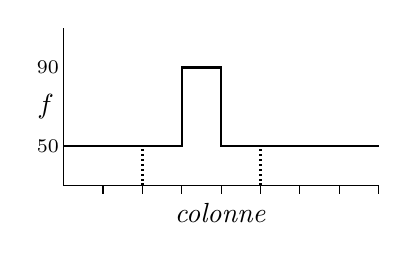
\begin{tikzpicture}[scale=1]
\draw (0,2) -- node[left] {$f$} (0,0) -- node[below,yshift=-1mm] {\textit{colonne}} (4,0);
\draw[thick] (0,.5) -- (1.5,.5) -- (1.5,1.5) -- (2,1.5) -- (2,.5) -- (4,.5);
\node at (-2mm,.5) {$\scriptstyle 50$};
\node at (-2mm,1.5) {$\scriptstyle 90$};
\foreach \x in {.5,1,1.5,2,2.5,3,3.5,4}
  \draw[thin] (\x,-1mm) -- (\x,0);
\draw[densely dotted,thick] (1,0) -- (1,.5);
\draw[densely dotted,thick] (2.5,0) -- (2.5,.5);
\end{tikzpicture}
\caption{Gráfico de intensidade antes de fazer a média}\label{fig.before-average}
\end{minipage}
\hspace{\fill}
\begin{minipage}{.47\textwidth}
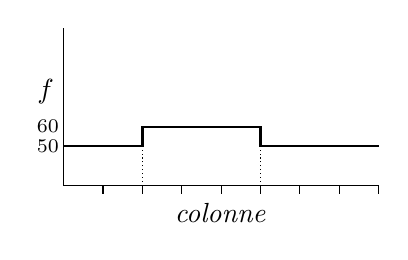
\begin{tikzpicture}[scale=1]
\draw (0,2) -- node[left,yshift=2mm] {$f$} (0,0) -- node[below,yshift=-1mm] {\textit{colonne}} (4,0);
\draw[thick] (0,.5) -- (1,.5) -- (1,.75) -- (2.5,.75) -- (2.5,.5) -- (4,.5);
\node at (-2mm,.5) {$\scriptstyle 50$};
\node at (-2mm,.75) {$\scriptstyle 60$};
\foreach \x in {.5,1,1.5,2,2.5,3,3.5,4}
  \draw[thin] (\x,-1mm) -- (\x,0);
\draw[densely dotted] (1,0) -- (1,.5);
\draw[densely dotted] (2.5,0) -- (2.5,.5);
\end{tikzpicture}
\caption{Gráfico de Intensidade após o cálculo da média}\label{fig.after-average}
\end{minipage}
\end{figure}

%\begin{figure}
%\subfigures
%\begin{minipage}{\textwidth}
%\leftfigure{
%\begin{tikzpicture}[scale=1.2]
%\draw (0,2) -- node[left] {$f$} (0,0) -- node[below,yshift=-1mm] {\textit{column}} (4,0);
%\draw[thick] (0,.5) -- (1.5,.5) -- (1.5,1.5) -- (2,1.5) -- (2,.5) -- (4,.5);
%\node at (-2mm,.5) {$\scriptstyle 50$};
%\node at (-2mm,1.5) {$\scriptstyle 90$};
%\foreach \x in {.5,1,1.5,2,2.5,3,3.5,4}
%  \draw[thin] (\x,-1mm) -- (\x,0);
%\draw[densely dotted,thick] (1,0) -- (1,.5);
%\draw[densely dotted,thick] (2.5,0) -- (2.5,.5);
%\end{tikzpicture}
%}
%\hspace{\fill}
%\rightfigure{
%\begin{tikzpicture}[scale=1.2]
%\draw (0,2) -- node[left,yshift=2mm] {$f$} (0,0) -- node[below,yshift=-1mm] {\textit{column}} (4,0);
%\draw[thick] (0,.5) -- (1,.5) -- (1,.75) -- (2.5,.75) -- (2.5,.5) -- (4,.5);
%\node at (-2mm,.5) {$\scriptstyle 50$};
%\node at (-2mm,.75) {$\scriptstyle 60$};
%\foreach \x in {.5,1,1.5,2,2.5,3,3.5,4}
%  \draw[thin] (\x,-1mm) -- (\x,0);
%\draw[densely dotted] (1,0) -- (1,.5);
%\draw[densely dotted] (2.5,0) -- (2.5,.5);
%\end{tikzpicture}
%}
%\leftcaption{Intensity plot before averaging}\label{fig.before-average}
%\rightcaption{Intensity plot after averaging}\label{fig.after-average}
%\end{minipage}
%\end{figure}

Taking the average of a sequence of pixels is the discrete version of integrating a continuous intensity function. Integration smooths out local variation of the function. The dotted lines in Figs.~\ref{fig.before-average}--\ref{fig.after-average} indicate a three-pixel sequence and it can be seen that the areas they bound are about the same.

The averaging operation is performed by applying a \emph{spatial filter} at each pixel of the image.\footnote{The mathematical term for applying a function $g$ at every point of a function $f$ is called (discrete) \emph{convolution}. For continuous functions integration is used in place of the addition of averaging.} For the two-dimensional array of pixels, the filter is represented by a $3\times 3$ array, where each element of the array specifies the factor by which the pixel and its neighbors are multiplied. Each pixel has four or eight neighbors, depending on whether we include the diagonal neighbors. Here, we include the diagonal pixels in the filters.

The \emph{box filter} is:
\[
\left[
\begin{array}{ccc}
1 & 1 & 1\\
1 & 1 & 1\\
1 & 1 & 1
\end{array}
\right]\,.
\]
The results of the multiplications are added and the sum is divided by $9$ to scale the result back to an intensity value.

The application of the filter to each pixel $(r,c)$ can be written explicitly as:
\[
\begin{array}{llll}
g(r,c) = &(\\
&f(r-1,c-1) & \;+\; f(r-1,c) & \;+\; f(r-1,c+1) \;+\\
&f(r,c-1) & \;+\; f(r,c) & \;+\; f(r,c+1) \;\;\;\;\;\;\;+\\
&f(r+1,c-1) & \;+\; f(r+1,c) & \;+\; f(r+1,c+1)\\
& ) \; / \; 9\,.
\end{array}
\]
The result of applying the box filter to the noisy image in Fig.~\ref{fig.pixel-noise} is shown in Fig.~\ref{fig.box-filter}.\footnote{The filter is not applied to the pixels in the boundary of the image to avoid exceeding the bounds of the array. Alternatively, the image can be padded with extra rows and columns.} The intensity values are no longer uniform but they are quite close to the original values, except where a noise pixels existed. The second row from the bottom shows that the noise value of $90$ no longer appears; instead, all the values in the row are close together in the range $46$--$54$.

\begin{figure}
\begin{minipage}{.5\textwidth}
\begin{tabular}{r@{\hspace{4pt}}r@{\hspace{4pt}}r@{\hspace{4pt}}r@{\hspace{4pt}}r@{\hspace{4pt}}r@{\hspace{4pt}}r@{\hspace{4pt}}r@{\hspace{4pt}}r@{\hspace{4pt}}r@{\hspace{4pt}}r}
& $\scriptstyle 0$ & $\scriptstyle 1$ & $\scriptstyle 2$ & $\scriptstyle 3$ & $\scriptstyle 4$ & $\scriptstyle 5$ & $\scriptstyle 6$ & $\scriptstyle 7$ & $\scriptstyle 8$ & $\scriptstyle 9$ \\
$\scriptstyle 0$ & 10 & 10 & 10 & 10 & 10 & 10 & 10 & 10 & 10 & 10\\
$\scriptstyle 1$ & 20 & 20 & 18 & 18 & 18 & 20 & 20 & 20 & 20 & 20\\
$\scriptstyle 2$ & 30 & 30 & 28 & 28 & 28 & 26 & 26 & 26 & 30 & 30\\
$\scriptstyle 3$ & 40 & 40 & 38 & 43 & 43 & 41 & 36 & 36 & 40 & 40\\
$\scriptstyle 4$ & 50 & 50 & 50 & 54 & 54 & 51 & 46 & 46 & 50 & 50\\
$\scriptstyle 5$ & 60 & 60 & 60 & 60 & 60 & 60 & 60 & 60 & 60 & 60\\
\end{tabular}
\caption{Sde alisamento com o filtro da caixa}\label{fig.box-filter}
\end{minipage}
\hspace{\fill}
\begin{minipage}{.5\textwidth}
\begin{tabular}{r@{\hspace{4pt}}r@{\hspace{4pt}}r@{\hspace{4pt}}r@{\hspace{4pt}}r@{\hspace{4pt}}r@{\hspace{4pt}}r@{\hspace{4pt}}r@{\hspace{4pt}}r@{\hspace{4pt}}r@{\hspace{4pt}}r}
& $\scriptstyle 0$ & $\scriptstyle 1$ & $\scriptstyle 2$ & $\scriptstyle 3$ & $\scriptstyle 4$ & $\scriptstyle 5$ & $\scriptstyle 6$ & $\scriptstyle 7$ & $\scriptstyle 8$ & $\scriptstyle 9$ \\
$\scriptstyle 0$ & 10 & 10 & 10 & 10 & 10 & 10 & 10 & 10 & 10 & 10\\
$\scriptstyle 1$ & 20 & 20 & 19 & 19 & 19 & 20 & 20 & 20 & 20 & 20\\
$\scriptstyle 2$ & 30 & 30 & 29 & 25 & 29 & 28 & 28 & 28 & 30 & 30\\
$\scriptstyle 3$ & 40 & 40 & 39 & 41 & 41 & 40 & 25 & 38 & 40 & 40\\
$\scriptstyle 4$ & 50 & 50 & 50 & 52 & 70 & 50 & 48 & 48 & 50 & 50\\
$\scriptstyle 5$ & 60 & 60 & 60 & 60 & 60 & 60 & 60 & 60 & 60 & 60\\
\end{tabular}
\caption{Alisamento com um filtro ponderado}\label{fig.weighted-filter}
\end{minipage}
\end{figure}


%\begin{figure}
%\subfigures
%\begin{minipage}{\textwidth}
%\leftfigure{
%\begin{tabular}{r@{\hspace{4pt}}r@{\hspace{6pt}}r@{\hspace{6pt}}r@{\hspace{6pt}}r@{\hspace{6pt}}r@{\hspace{6pt}}r@{\hspace{6pt}}r@{\hspace{6pt}}r@{\hspace{6pt}}r@{\hspace{6pt}}r}
%& $\scriptstyle 0$ & $\scriptstyle 1$ & $\scriptstyle 2$ & $\scriptstyle 3$ & $\scriptstyle 4$ & $\scriptstyle 5$ & $\scriptstyle 6$ & $\scriptstyle 7$ & $\scriptstyle 8$ & $\scriptstyle 9$ \\
%$\scriptstyle 0$ & 10 & 10 & 10 & 10 & 10 & 10 & 10 & 10 & 10 & 10\\
%$\scriptstyle 1$ & 20 & 20 & 18 & 18 & 18 & 20 & 20 & 20 & 20 & 20\\
%$\scriptstyle 2$ & 30 & 30 & 28 & 28 & 28 & 26 & 26 & 26 & 30 & 30\\
%$\scriptstyle 3$ & 40 & 40 & 38 & 43 & 43 & 41 & 36 & 36 & 40 & 40\\
%$\scriptstyle 4$ & 50 & 50 & 50 & 54 & 54 & 51 & 46 & 46 & 50 & 50\\
%$\scriptstyle 5$ & 60 & 60 & 60 & 60 & 60 & 60 & 60 & 60 & 60 & 60\\
%\end{tabular}
%}
%\hspace{\fill}
%\rightfigure{
%\begin{tabular}{r@{\hspace{4pt}}r@{\hspace{6pt}}r@{\hspace{6pt}}r@{\hspace{6pt}}r@{\hspace{6pt}}r@{\hspace{6pt}}r@{\hspace{6pt}}r@{\hspace{6pt}}r@{\hspace{6pt}}r@{\hspace{6pt}}r}
%& $\scriptstyle 0$ & $\scriptstyle 1$ & $\scriptstyle 2$ & $\scriptstyle 3$ & $\scriptstyle 4$ & $\scriptstyle 5$ & $\scriptstyle 6$ & $\scriptstyle 7$ & $\scriptstyle 8$ & $\scriptstyle 9$ \\
%$\scriptstyle 0$ & 10 & 10 & 10 & 10 & 10 & 10 & 10 & 10 & 10 & 10\\
%$\scriptstyle 1$ & 20 & 20 & 19 & 19 & 19 & 20 & 20 & 20 & 20 & 20\\
%$\scriptstyle 2$ & 30 & 30 & 29 & 25 & 29 & 28 & 28 & 28 & 30 & 30\\
%$\scriptstyle 3$ & 40 & 40 & 39 & 41 & 41 & 40 & 25 & 38 & 40 & 40\\
%$\scriptstyle 4$ & 50 & 50 & 50 & 52 & 70 & 50 & 48 & 48 & 50 & 50\\
%$\scriptstyle 5$ & 60 & 60 & 60 & 60 & 60 & 60 & 60 & 60 & 60 & 60\\
%\end{tabular}
%}
%\leftcaption{Smoothing with the box filter}\label{fig.box-filter}
%\rightcaption{Smoothing with a weighted filter}\label{fig.weighted-filter}
%\end{minipage}
%\end{figure}

The box filter gives equal importance to the pixel and all its neighbors, but a \emph{weighted filter} uses different factors for different pixels. The following filter gives much more weight to the pixel itself than to its neighbors:
\[
\left[
\begin{array}{ccc}
1 & 1 & 1\\
1 & 8 & 1\\
1 & 1 & 1
\end{array}
\right]\,.
\]
It would be appropriate to use this filter if we think that a pixel almost certainly has its correct value, but we still want its neighbors to influence its value. After applying this filter, the result must be divided by $16$ to scale the sum to an intensity value. Figure~\ref{fig.weighted-filter} shows the result of using the weighted filter. Looking again at the second row from the bottom, the value of $90$ has only been reduced to $70$ because greater weight is given to the pixel relative to its neighbors.

\begin{framed}
\act{Image enhancement: smoothing}{smoothing}
\begin{itemize}
\item Print a sheet of paper with a gray-level pattern like the one shown in Fig.~\ref{fig.one-enhance}. The pattern has two black lines that we wish to detect but also three dark-gray areas (indicated by the arrows) that are likely to be incorrectly detected as lines.
\item Program the robot so that it moves from left to right over the pattern, sampling the output of the ground sensor. Examine the output and set a threshold so that the robot detects both the black lines and the dark-gray areas. Modify the program so that in its second pass, it indicates (by light or sound) when it has detected a black line and a dark area.
\item Modify the program so that it replaces every sample by the average of the intensity of the sample and its two neighbors. The robot should now detect the two black lines but not the gray areas.
\item Experiment with different weights for the average.
\item Experiment with different sampling rates. What happens if you sample the ground sensor at very short intervals?
\end{itemize}
\end{framed}

\begin{figure}
\begin{center}
\begin{tikzpicture}
\pic at (-2,1.5) { robot };
\draw[fill,gray] (-1,1.3) rectangle +(6pt,12pt);
\foreach \n/\colorb/\colort in
  {-.5/40/50, 0/50/70, .5/70/40, 1/40/50, 1.5/50/70, 2.0/70/50, 2.5/50/40,%
   4/40/50, 4.5/50/70, 5/70/50, 5.5/50/40,%
   7/40/50, 7.5/50/40, 8/40/40}
    \shade[left color=black!\colorb,right color=black!\colort] (\n,0) rectangle +(5mm,3);
\foreach \x in {.5,2,5}
  \draw[->] (\x, -.4) -- (\x, -.1);
\draw[fill,color=black] (3,0) rectangle +(1,3);
\draw[fill,color=black] (6,0) rectangle +(1,3);
\end{tikzpicture}
\caption{One-dimensional image enhancement}\label{fig.one-enhance}
\end{center}
\end{figure}

\subsection{Histogram manipulation}

Figure~\ref{fig.binary-no-noise} shows the pixels of a binary image: an image where each pixel is either black or white.\footnote{The values $10$ for black and $90$ for white have been used instead of the more usual $0$ and $100$ for clarity in printing the array.} The image shows a $3\times 5$ white rectangle on the black background. Figure~\ref{fig.binary-noise} shows the same image with a lot of random noise added. By looking at the image it is possible to identify the rectangle, but it is very difficult to do and smoothing the image won't help.

\begin{figure}
\begin{minipage}{.5\textwidth}
\begin{tabular}{r@{\hspace{4pt}}r@{\hspace{4pt}}r@{\hspace{4pt}}r@{\hspace{4pt}}r@{\hspace{4pt}}r@{\hspace{4pt}}r@{\hspace{4pt}}r@{\hspace{4pt}}r@{\hspace{4pt}}r@{\hspace{4pt}}r}
& $\scriptstyle 0$ & $\scriptstyle 1$ & $\scriptstyle 2$ & $\scriptstyle 3$ & $\scriptstyle 4$ & $\scriptstyle 5$ & $\scriptstyle 6$ & $\scriptstyle 7$ & $\scriptstyle 8$ & $\scriptstyle 9$ \\
$\scriptstyle 0$ & $10$ & $10$ & $10$ & $10$ & $10$ & $10$ & $10$ & $10$ & $10$ & $10$\\
$\scriptstyle 1$ & $10$ & $10$ & $10$ & $10$ & $10$ & $10$ & $10$ & $10$ & $10$ & $10$\\
$\scriptstyle 2$ & $10$ & $10$ & $10$ & \boldmath $90$ & \boldmath $90$ & \boldmath $90$ & \boldmath $90$ & \boldmath $90$ & $10$ & $10$\\
$\scriptstyle 3$ & $10$ & $10$ & $10$ & \boldmath $90$ & \boldmath $90$ & \boldmath $90$ & \boldmath $90$ & \boldmath $90$ & $10$ & $10$\\
$\scriptstyle 4$ & $10$ & $10$ & $10$ & \boldmath $90$ & \boldmath $90$ & \boldmath $90$ & \boldmath $90$ & \boldmath $90$ & $10$ & $10$\\
$\scriptstyle 5$ & $10$ & $10$ & $10$ & $10$ & $10$ & $10$ & $10$ & $10$ & $10$ & $10$\\
\end{tabular}
\caption{Imagem binária sem ruído}\label{fig.binary-no-noise}\end{minipage}
\hspace{\fill}
\begin{minipage}{.5\textwidth}
\begin{tabular}{r@{\hspace{4pt}}r@{\hspace{4pt}}r@{\hspace{4pt}}r@{\hspace{4pt}}r@{\hspace{4pt}}r@{\hspace{4pt}}r@{\hspace{4pt}}r@{\hspace{4pt}}r@{\hspace{4pt}}r@{\hspace{4pt}}r}
& $\scriptstyle 0$ & $\scriptstyle 1$ & $\scriptstyle 2$ & $\scriptstyle 3$ & $\scriptstyle 4$ & $\scriptstyle 5$ & $\scriptstyle 6$ & $\scriptstyle 7$ & $\scriptstyle 8$ & $\scriptstyle 9$ \\
$\scriptstyle 0$ & $19$ & $17$ & $37$ & $19$ & $26$ & $11$ & $46$ & $27$ & $37$ & $10$\\
$\scriptstyle 1$ & $11$ & $24$ & $17$ & $30$ & $14$ & $43$ & $29$ & $22$ & $34$ & $46$\\
$\scriptstyle 2$ & $31$ & $37$ & $38$ & $63$ & $72$ & $86$ & $65$ & $64$ & $27$ & $47$\\
$\scriptstyle 3$ & $33$ & $38$ & $49$ & $73$ & $63$ & $66$ & $59$ & $76$ & $40$ & $10$\\
$\scriptstyle 4$ & $47$ & $13$ & $44$ & $90$ & $86$ & $56$ & $63$ & $65$ & $18$ & $44$\\
$\scriptstyle 5$ & $10$ & $34$ & $29$ & $14$ & $35$ & $31$ & $26$ & $42$ & $15$ & $25$\\
\end{tabular}
\caption{Imagem binária com ruído}\label{fig.binary-noise}
\end{minipage}
\end{figure}

%\begin{figure}
%\subfigures
%\begin{minipage}{\textwidth}
%\leftfigure{
%\begin{tabular}{r@{\hspace{4pt}}r@{\hspace{6pt}}r@{\hspace{6pt}}r@{\hspace{6pt}}r@{\hspace{6pt}}r@{\hspace{6pt}}r@{\hspace{6pt}}r@{\hspace{6pt}}r@{\hspace{6pt}}r@{\hspace{6pt}}r}
%& $\scriptstyle 0$ & $\scriptstyle 1$ & $\scriptstyle 2$ & $\scriptstyle 3$ & $\scriptstyle 4$ & $\scriptstyle 5$ & $\scriptstyle 6$ & $\scriptstyle 7$ & $\scriptstyle 8$ & $\scriptstyle 9$ \\
%$\scriptstyle 0$ & $10$ & $10$ & $10$ & $10$ & $10$ & $10$ & $10$ & $10$ & $10$ & $10$\\
%$\scriptstyle 1$ & $10$ & $10$ & $10$ & $10$ & $10$ & $10$ & $10$ & $10$ & $10$ & $10$\\
%$\scriptstyle 2$ & $10$ & $10$ & $10$ & \boldmath $90$ & \boldmath $90$ & \boldmath $90$ & \boldmath $90$ & \boldmath $90$ & $10$ & $10$\\
%$\scriptstyle 3$ & $10$ & $10$ & $10$ & \boldmath $90$ & \boldmath $90$ & \boldmath $90$ & \boldmath $90$ & \boldmath $90$ & $10$ & $10$\\
%$\scriptstyle 4$ & $10$ & $10$ & $10$ & \boldmath $90$ & \boldmath $90$ & \boldmath $90$ & \boldmath $90$ & \boldmath $90$ & $10$ & $10$\\
%$\scriptstyle 5$ & $10$ & $10$ & $10$ & $10$ & $10$ & $10$ & $10$ & $10$ & $10$ & $10$\\
%\end{tabular}
%}
%\hspace{\fill}
%\rightfigure{
%\begin{tabular}{r@{\hspace{4pt}}r@{\hspace{6pt}}r@{\hspace{6pt}}r@{\hspace{6pt}}r@{\hspace{6pt}}r@{\hspace{6pt}}r@{\hspace{6pt}}r@{\hspace{6pt}}r@{\hspace{6pt}}r@{\hspace{6pt}}r}
%& $\scriptstyle 0$ & $\scriptstyle 1$ & $\scriptstyle 2$ & $\scriptstyle 3$ & $\scriptstyle 4$ & $\scriptstyle 5$ & $\scriptstyle 6$ & $\scriptstyle 7$ & $\scriptstyle 8$ & $\scriptstyle 9$ \\
%$\scriptstyle 0$ & $19$ & $17$ & $37$ & $19$ & $26$ & $11$ & $46$ & $27$ & $37$ & $10$\\
%$\scriptstyle 1$ & $11$ & $24$ & $17$ & $30$ & $14$ & $43$ & $29$ & $22$ & $34$ & $46$\\
%$\scriptstyle 2$ & $31$ & $37$ & $38$ & $63$ & $72$ & $86$ & $65$ & $64$ & $27$ & $47$\\
%$\scriptstyle 3$ & $33$ & $38$ & $49$ & $73$ & $63$ & $66$ & $59$ & $76$ & $40$ & $10$\\
%$\scriptstyle 4$ & $47$ & $13$ & $44$ & $90$ & $86$ & $56$ & $63$ & $65$ & $18$ & $44$\\
%$\scriptstyle 5$ & $10$ & $34$ & $29$ & $14$ & $35$ & $31$ & $26$ & $42$ & $15$ & $25$\\
%\end{tabular}
%}
%\leftcaption{Binary image without noise}\label{fig.binary-no-noise}
%\rightcaption{Binary image with noise}\label{fig.binary-noise}
%\end{minipage}
%\end{figure}

Let us now construct a \emph{histogram} of the intensities (Fig.~\ref{fig.hist}). A histogram is constructed of \emph{bins}, where each bin stores a count of the pixels having a range of intensities. The histogram in the figure contains ten bins for intensities in the ranges $0$--$9$, $10$--$19$, \ldots, $91$--$99$. If we assume that the white rectangle is small relative to the background, it is easy to see from the histogram that there are two groups of pixels, those that are relatively dark and those that are relatively bright. A threshold of $50$ or $60$ should be able to distinguish between the rectangle and the background even in the presence of noise. In fact, a threshold of $50$ restores the original image, while a threshold of $60$ correctly restores $13$ of the $15$ pixels of the rectangle.

\begin{figure}
\begin{center}
\begin{tikzpicture}
\draw (0,2) -- node[left,xshift=-2mm] {\textit{count}} (0,0) -- node[below,yshift=-5mm] {\textit{intensity}} (10,0);
\foreach \n/\v/\y/\lab in {0/0/0/0--9, 1/14/1.4/10--19, 2/9/.9/20--29, 3/12/1.2/30--39, 4/10/1/40--49, 5/2/.2/50--59, 6/7/.7/60--69, 7/3/.3/70--79, 8/2/.2/80--89, 9/1/.1/90--99}
  \pic { barhist=\n/\v/\y/\lab };
\end{tikzpicture}
\caption{Histogram of the noisy image}\label{fig.hist}
\end{center}
\end{figure}

The advantage of histogram manipulation is that it is very efficient to compute even on large images. For each pixel, divide the intensity by the number of bins and increment the bin number:
\begin{quote}
\p{for each pixel p}\\
\hspace*{2em}\p{bin\_number} $\leftarrow$ \p{intensity(p) / number\_of\_bins}\\
\hspace*{2em}\p{bins[bin\_number]} $\leftarrow$ \p{bins[bin\_number] + 1}
\end{quote}
Compare this operation with the application of a $3\times 3$ spatial filter which requires $9$ multiplications, $8$ additions and a division at each pixel. Furthermore, little memory is needed. We chose $10$ bins so that Fig.~\ref{fig.hist} could display the entire histogram, but a full $8$-bit grayscale histogram requires only $256$ bins.

Choosing a threshold by examining a plot of the histogram is easy, and if you know roughly the fraction of the background covered by objects, the selection of the threshold can be done automatically.

Algorithms for histogram manipulation can perform more complex enhancement than the simple binary threshold we described here. In particular, there are algorithms for enhancing images by modifying the brightness and contrast of an image. 

\begin{framed}
\act{Image enhancement: histogram manipulation}{hist}
\begin{itemize}
\item Modify the program in Activity~\ref{act.smoothing} so that it computes the histogram of the samples.
\item How does the histogram change if the number of samples is increased?
\item Examine the histogram to determine a threshold that will be used to distinguish between the black lines and the background.
\item Compute the sum of the contents of the bins until the sum is greater than a fraction (perhaps one-third) of the samples. Use the index of the last bin to set the threshold.
\end{itemize}
\end{framed}

\section{Edge detection}\label{s.edge-detection}

Medical image processing systems need sophisticated image enhancement algorithms for modifying brightness and contrast, removing noise, etc. However, once the image is enhanced, interpretation of the image is performed by specialists who know which lines and shadows correspond with which organs in the body, and if the organs are normal or not. An autonomous robot does not have a human to perform interpretation: it needs to identify objects such as doors in a building, boxes in a warehouse and cars on the road. The first step is to extract features or segments such as lines, edges and areas.

\begin{figure}
\begin{minipage}{.5\textwidth}
\begin{tabular}{r@{\hspace{4pt}}r@{\hspace{6pt}}r@{\hspace{6pt}}r@{\hspace{6pt}}r@{\hspace{6pt}}r@{\hspace{6pt}}r@{\hspace{6pt}}r@{\hspace{6pt}}r@{\hspace{6pt}}r@{\hspace{6pt}}r}
& $\scriptstyle 0$ & $\scriptstyle 1$ & $\scriptstyle 2$ & $\scriptstyle 3$ & $\scriptstyle 4$ & $\scriptstyle 5$\\
$\scriptstyle 0$ & $30$ & $30$ & $30$ & $30$ & $30$ &$30$\\
$\scriptstyle 1$ & $30$ & $30$ & $30$ & $30$ & $30$ &$30$\\
$\scriptstyle 2$ & $30$ & $30$ & $30$ & $30$ & $30$ &$30$\\
$\scriptstyle 3$ & \boldmath $50$ & \boldmath $50$ & \boldmath $50$ & \boldmath $50$ & \boldmath $50$ & \boldmath $50$\\
$\scriptstyle 4$ & \boldmath $50$ & \boldmath $50$ & \boldmath $50$ & \boldmath $50$ & \boldmath $50$ & \boldmath $50$\\
$\scriptstyle 5$ & \boldmath $50$ & \boldmath $50$ & \boldmath $50$ & \boldmath $50$ & \boldmath $50$ & \boldmath $50$\\
\end{tabular}
\caption{Imagem com uma borda}\label{fig.edge}
\end{minipage}
\hspace{\fill}
\begin{minipage}{.5\textwidth}
\begin{tikzpicture}[scale=1.5,baseline=-18mm]
\draw (0,1) -- node[left] {$f$} (0,0) -- node[below,yshift=-2mm] {\textit{rangée}} (3,0);
\draw[thick] (0,.25) -- (1.5,.25) -- (2,.75) -- (3,.75);
\node at (-1.5mm,.2) {\scriptsize{30}};
\node at (-1.5mm,.8) {\scriptsize{50}};
\foreach \x in {.5,1,1.5,2,2.5,3}
  \draw[thin] (\x,-1mm) -- (\x,0);
\end{tikzpicture}
\caption{Intensidade da borda}\label{fig.edge-intensity}
\end{minipage}
\end{figure}

%\begin{figure}
%\subfigures
%\begin{minipage}{\textwidth}
%\leftfigure{
%\begin{tabular}{r@{\hspace{4pt}}r@{\hspace{6pt}}r@{\hspace{6pt}}r@{\hspace{6pt}}r@{\hspace{6pt}}r@{\hspace{6pt}}r@{\hspace{6pt}}r@{\hspace{6pt}}r@{\hspace{6pt}}r@{\hspace{6pt}}r}
%& $\scriptstyle 0$ & $\scriptstyle 1$ & $\scriptstyle 2$ & $\scriptstyle 3$ & $\scriptstyle 4$ & $\scriptstyle 5$\\
%$\scriptstyle 0$ & $30$ & $30$ & $30$ & $30$ & $30$ &$30$\\
%$\scriptstyle 1$ & $30$ & $30$ & $30$ & $30$ & $30$ &$30$\\
%$\scriptstyle 2$ & $30$ & $30$ & $30$ & $30$ & $30$ &$30$\\
%$\scriptstyle 3$ & \boldmath $50$ & \boldmath $50$ & \boldmath $50$ & \boldmath $50$ & \boldmath $50$ & \boldmath $50$\\
%$\scriptstyle 4$ & \boldmath $50$ & \boldmath $50$ & \boldmath $50$ & \boldmath $50$ & \boldmath $50$ & \boldmath $50$\\
%$\scriptstyle 5$ & \boldmath $50$ & \boldmath $50$ & \boldmath $50$ & \boldmath $50$ & \boldmath $50$ & \boldmath $50$\\
%\end{tabular}
%}
%\hspace{\fill}
%\rightfigure{
%\begin{tikzpicture}[scale=1.7]
%\draw (0,1) -- node[left] {$f$} (0,0) -- node[below,yshift=-2mm] {\textit{row}} (3,0);
%\draw[thick] (0,.25) -- (1.5,.25) -- (2,.75) -- (3,.75);
%\node at (-1.5mm,.2) {\scriptsize{30}};
%\node at (-1.5mm,.8) {\scriptsize{50}};
%\foreach \x in {.5,1,1.5,2,2.5,3}
%  \draw[thin] (\x,-1mm) -- (\x,0);
%\end{tikzpicture}
%}
%\leftcaption{Image with an edge}\label{fig.edge}
%\rightcaption{Intensity of edge}\label{fig.edge-intensity}
%\end{minipage}
%\end{figure}

Consider the $6\times 6$ array of pixels in Fig.~\ref{fig.edge}. The intensity level of each row is uniform but there is a sharp discontinuity between the intensity level of rows $2$ and $3$. Clearly, this represents an edge between the dark area at the top and the light area at the bottom. Averaging will make the intensity change smoother and we lose the sharp change at the edge.

\begin{figure}
\begin{minipage}{.5\textwidth}
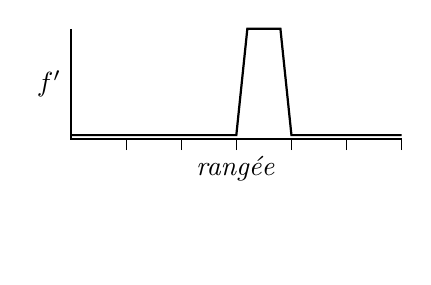
\begin{tikzpicture}[scale=1.4,baseline=-1.5cm]
\draw (0,1) -- node[left] {$f'$} (0,0) -- node[below,yshift=-1mm] {\textit{rangée}} (3,0);
\draw[thick] (0,1pt) -- (1.5,1pt) -- (1.6,1) -- (1.9,1) -- (2,1pt) -- (3,1pt);
\foreach \x in {.5,1,1.5,2,2.5,3}
  \draw[thin] (\x,-1mm) -- (\x,0);
\end{tikzpicture}
\caption{Primeira derivada de intensidade de borda}
\label{fig.edge-first}
\end{minipage}
\hspace{\fill}
\begin{minipage}{.5\textwidth}
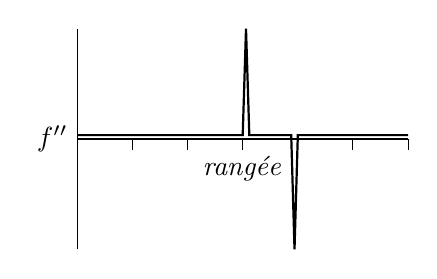
\begin{tikzpicture}[scale=1.4]
\draw (0,-1) -- node[left] {$f''$} (0,1);
\draw (0,0) -- node[below,yshift=-1mm] {\textit{rangée}} (3,0);
\draw[thick] (0,1pt) -- (1.5,1pt) -- (1.53,1) -- (1.56,1pt) -- (1.94,1pt) -- (1.97,-1) -- (2,1pt) -- (3,1pt);
\foreach \x in {.5,1,1.5,2,2.5,3}
  \draw[thin] (\x,-1mm) -- (\x,0);
\end{tikzpicture}
\caption{Second derivative of edge intensity}\label{fig.edge-second}
\end{minipage}
\end{figure}

%\begin{figure}
%\subfigures
%\begin{minipage}{\textwidth}
%\leftfigure{
%\begin{tikzpicture}[scale=1.6,baseline=-1.5cm]
%\draw (0,1) -- node[left] {$f'$} (0,0) -- node[below,yshift=-1mm] {\textit{row}} (3,0);
%\draw[thick] (0,1pt) -- (1.5,1pt) -- (1.6,1) -- (1.9,1) -- (2,1pt) -- (3,1pt);
%\foreach \x in {.5,1,1.5,2,2.5,3}
%  \draw[thin] (\x,-1mm) -- (\x,0);
%\end{tikzpicture}
%}
%\hspace{\fill}
%\rightfigure{
%\begin{tikzpicture}[scale=1.6]
%\draw (0,-1) -- node[left] {$f''$} (0,1);
%\draw (0,0) -- node[below,yshift=-1mm] {\textit{row}} (3,0);
%\draw[thick] (0,1pt) -- (1.5,1pt) -- (1.53,1) -- (1.56,1pt) -- (1.94,1pt) -- (1.97,-1) -- (2,1pt) -- (3,1pt);
%\foreach \x in {.5,1,1.5,2,2.5,3}
%  \draw[thin] (\x,-1mm) -- (\x,0);
%\end{tikzpicture}
%}
%\leftcaption{First derivative of edge intensity}\label{fig.edge-first}
%\rightcaption{Second derivative of edge intensity}\label{fig.edge-second}
%\end{minipage}
%\end{figure}

Since averaging is an integrating operator that \emph{removes} abrupt changes in intensities, it is not surprising that the differential operator can be used to \emph{detect} abrupt changes that represent edges. Figure~\ref{fig.edge-intensity} plots the intensity against the row number along a single column of Fig.~\ref{fig.edge}, although the intensities are shown as lines instead of as discrete points. The intensity doesn't change for the first three pixels, then it rapidly increases and continues at the higher level. The first derivative $f'$ of a function $f$ is zero when $f$ is constant, positive when $f$ increases and negative when $f$ decreases. This is shown in Fig.~\ref{fig.edge-first}. An edge can be detected by searching for a rapid increase or decrease of the first derivative of the image intensity.

In practice, it is better to use the second derivative. Figure~\ref{fig.edge-second} shows a plot of $f''$, the derivative of $f'$ in Fig.~\ref{fig.edge-first}. The positive spike followed by the negative spike indicates a transition from dark to light; if the transition were from light to dark, the negative spike would precede the positive spike.

There are many digital derivative operators. A simple but effective one is the \emph{Sobel filter}. There are two filters, one for detecting horizontal edges (on the left) and other for detecting vertical edges (on the right):
\[
\begin{array}{c@{\hspace{4em}}c}
\left[
\begin{array}{rrr}
-1 & -2 & -1\\
0 & 0 & 0\\
1 & 2 & 1\\
\end{array}
\right]
&
\left[
\begin{array}{rrr}
-1 & 0 & 1\\
-2 & 0 & 2\\
-1 & 0 & 1\\
\end{array}
\right]\,.
\end{array}
\]
A characteristic of a derivative filter is that the sum of its elements must equal zero. The reason is that if the operator is applied to a pixel whose intensity is the same as that of all its neighbors, the result must be zero. Look again at Figs.~\ref{fig.edge-intensity} and~\ref{fig.edge-first} where the derivative is zero when the intensity is constant.

When the Sobel filters are applied to the pixel array in Fig.~\ref{fig.edge}, the result clearly detects that there is a horizontal edge (Fig.~\ref{fig.sobel-horizontal}) but no vertical edge (Fig.~\ref{fig.sobel-vertical}).

\begin{figure}
\begin{minipage}{.45\textwidth}
\begin{tabular}{r@{\hspace{4pt}}r@{\hspace{6pt}}r@{\hspace{6pt}}r@{\hspace{6pt}}r@{\hspace{6pt}}r@{\hspace{6pt}}r@{\hspace{6pt}}r@{\hspace{6pt}}r@{\hspace{6pt}}r@{\hspace{6pt}}r}
& $\scriptstyle 0$ & $\scriptstyle 1$ & $\scriptstyle 2$ & $\scriptstyle 3$ & $\scriptstyle 4$ & $\scriptstyle 5$\\
$\scriptstyle 0$ &    $0$ &   $0$ &   $0$ &   $0$ &   $0$ &   $0$ \\
$\scriptstyle 1$ &    $0$ &   $0$ &   $0$ &   $0$ &   $0$ &   $0$ \\
$\scriptstyle 2$ &    $0$ &  $80$ &  $80$ &  $80$ &  $80$ &   $0$ \\
$\scriptstyle 3$ &    $0$ &  $80$ &  $80$ &  $80$ &  $80$ &   $0$ \\
$\scriptstyle 4$ &    $0$ &   $0$ &   $0$ &   $0$ &   $0$ &   $0$ \\
$\scriptstyle 5$ &    $0$ &   $0$ &   $0$ &   $0$ &   $0$ &   $0$ \\
\end{tabular}
\caption{Borda horizontal Sobel}\label{fig.sobel-horizontal}
\end{minipage}
\hspace{\fill}
\begin{minipage}{.45\textwidth}
\begin{tabular}{r@{\hspace{4pt}}r@{\hspace{6pt}}r@{\hspace{6pt}}r@{\hspace{6pt}}r@{\hspace{6pt}}r@{\hspace{6pt}}r@{\hspace{6pt}}r@{\hspace{6pt}}r@{\hspace{6pt}}r@{\hspace{6pt}}r}
& $\scriptstyle 0$ & $\scriptstyle 1$ & $\scriptstyle 2$ & $\scriptstyle 3$ & $\scriptstyle 4$ & $\scriptstyle 5$\\
$\scriptstyle 0$ &    $0$ &   $0$ &   $0$ &   $0$ &   $0$ &   $0$ \\
$\scriptstyle 1$ &    $0$ &   $0$ &   $0$ &   $0$ &   $0$ &   $0$ \\
$\scriptstyle 2$ &    $0$ &   $0$ &   $0$ &   $0$ &   $0$ &   $0$ \\
$\scriptstyle 3$ &    $0$ &   $0$ &   $0$ &   $0$ &   $0$ &   $0$ \\
$\scriptstyle 4$ &    $0$ &   $0$ &   $0$ &   $0$ &   $0$ &   $0$ \\
$\scriptstyle 5$ &    $0$ &   $0$ &   $0$ &   $0$ &   $0$ &   $0$ \\
\end{tabular}
\caption{Borda vertical Sobel}\label{fig.sobel-vertical}
\end{minipage}
\end{figure}


%\begin{figure}
%\subfigures
%\begin{minipage}{\textwidth}
%\leftfigure{
%\begin{tabular}{r@{\hspace{4pt}}r@{\hspace{6pt}}r@{\hspace{6pt}}r@{\hspace{6pt}}r@{\hspace{6pt}}r@{\hspace{6pt}}r@{\hspace{6pt}}r@{\hspace{6pt}}r@{\hspace{6pt}}r@{\hspace{6pt}}r}
%& $\scriptstyle 0$ & $\scriptstyle 1$ & $\scriptstyle 2$ & $\scriptstyle 3$ & $\scriptstyle 4$ & $\scriptstyle 5$\\
%$\scriptstyle 0$ &    $0$ &   $0$ &   $0$ &   $0$ &   $0$ &   $0$ \\
%$\scriptstyle 1$ &    $0$ &   $0$ &   $0$ &   $0$ &   $0$ &   $0$ \\
%$\scriptstyle 2$ &    $0$ &  $80$ &  $80$ &  $80$ &  $80$ &   $0$ \\
%$\scriptstyle 3$ &    $0$ &  $80$ &  $80$ &  $80$ &  $80$ &   $0$ \\
%$\scriptstyle 4$ &    $0$ &   $0$ &   $0$ &   $0$ &   $0$ &   $0$ \\
%$\scriptstyle 5$ &    $0$ &   $0$ &   $0$ &   $0$ &   $0$ &   $0$ \\
%\end{tabular}
%}
%\hspace{\fill}
%\rightfigure{
%\begin{tabular}{r@{\hspace{4pt}}r@{\hspace{6pt}}r@{\hspace{6pt}}r@{\hspace{6pt}}r@{\hspace{6pt}}r@{\hspace{6pt}}r@{\hspace{6pt}}r@{\hspace{6pt}}r@{\hspace{6pt}}r@{\hspace{6pt}}r}
%& $\scriptstyle 0$ & $\scriptstyle 1$ & $\scriptstyle 2$ & $\scriptstyle 3$ & $\scriptstyle 4$ & $\scriptstyle 5$\\
%$\scriptstyle 0$ &    $0$ &   $0$ &   $0$ &   $0$ &   $0$ &   $0$ \\
%$\scriptstyle 1$ &    $0$ &   $0$ &   $0$ &   $0$ &   $0$ &   $0$ \\
%$\scriptstyle 2$ &    $0$ &   $0$ &   $0$ &   $0$ &   $0$ &   $0$ \\
%$\scriptstyle 3$ &    $0$ &   $0$ &   $0$ &   $0$ &   $0$ &   $0$ \\
%$\scriptstyle 4$ &    $0$ &   $0$ &   $0$ &   $0$ &   $0$ &   $0$ \\
%$\scriptstyle 5$ &    $0$ &   $0$ &   $0$ &   $0$ &   $0$ &   $0$ \\
%\end{tabular}
%}
%\leftcaption{Sobel horizontal edge}\label{fig.sobel-horizontal}
%\rightcaption{Sobel vertical edge}\label{fig.sobel-vertical}
%\end{minipage}
%\end{figure}

Sobel filters are very powerful because they can not only detect an edge but also compute the angle of the edge within the image. Figure~\ref{fig.diagonal-edge} shows an image with an edge running diagonally from the upper left to the lower right. The results of applying the two Sobel filters are shown in Figs.~\ref{fig.sobel-diagonal-horizontal}--\ref{fig.sobel-diagonal-vertical}. From the magnitudes and signs of the elements of these arrays, the angle of the edge can be computed as described in \cite[Sect.~4.3.1]{siegwart}.

\begin{figure}
\begin{tabular}{r@{\hspace{4pt}}r@{\hspace{6pt}}r@{\hspace{6pt}}r@{\hspace{6pt}}r@{\hspace{6pt}}r@{\hspace{6pt}}r@{\hspace{6pt}}r@{\hspace{6pt}}r@{\hspace{6pt}}r@{\hspace{6pt}}r}
& $\scriptstyle 0$ & $\scriptstyle 1$ & $\scriptstyle 2$ & $\scriptstyle 3$ & $\scriptstyle 4$ & $\scriptstyle 5$\\
$\scriptstyle 0$ &    $30$ &   $30$ &   $30$ &   $30$ &   $30$ & $30$ \\
$\scriptstyle 1$ &    \boldmath $50$ &   $30$ &   $30$ &   $30$ &   $30$ & $30$ \\
$\scriptstyle 2$ &    \boldmath $50$ &   \boldmath 50$$ &   $30$ &   $30$ &   $30$ & $30$ \\
$\scriptstyle 3$ &    \boldmath $50$ &   \boldmath $50$ &   \boldmath $50$ &   $30$ &   $30$ & $30$ \\
$\scriptstyle 4$ &    \boldmath $50$ &   \boldmath $50$ &   \boldmath $50$ &   \boldmath $50$ &   $30$ & $30$ \\
$\scriptstyle 5$ &    \boldmath $50$ &   \boldmath $50$ &   \boldmath $50$ &   \boldmath $50$ &   \boldmath $50$ & $30$ \\
\end{tabular}
\caption{Diagonal edge}\label{fig.diagonal-edge}
\end{figure}

\begin{figure}
\begin{minipage}{.45\textwidth}
\begin{tabular}{r@{\hspace{4pt}}r@{\hspace{6pt}}r@{\hspace{6pt}}r@{\hspace{6pt}}r@{\hspace{6pt}}r@{\hspace{6pt}}r@{\hspace{6pt}}r@{\hspace{6pt}}r@{\hspace{6pt}}r@{\hspace{6pt}}r}
& $\scriptstyle 0$ & $\scriptstyle 1$ & $\scriptstyle 2$ & $\scriptstyle 3$ & $\scriptstyle 4$ & $\scriptstyle 5$\\
$\scriptstyle 0$ &    $0$ &   $0$ &   $0$ &   $0$ &   $0$ &   $0$ \\
$\scriptstyle 1$ &    $0$ &   \boldmath $60$ &   $20$ &   $0$ &   $0$ &   $0$ \\
$\scriptstyle 2$ &    $0$ &   \boldmath $60$ &   \boldmath $60$ &   $20$ &   $0$ &   $0$ \\
$\scriptstyle 3$ &    $0$ &   $20$ &   \boldmath $60$ &   \boldmath $60$ &   $20$ &   $0$ \\
$\scriptstyle 4$ &    $0$ &   $0$ &   $20$ &   \boldmath $60$ &   \boldmath $60$ &   $0$ \\
$\scriptstyle 5$ &    $0$ &   $0$ &   $0$ &   $0$ &   $0$ &   $0$ \\
\end{tabular}
\caption{Filtro horizontal Sobel em uma borda diagonal}\label{fig.sobel-diagonal-horizontal}
\end{minipage}
\hspace{\fill}
\begin{minipage}{.45\textwidth}
\begin{tabular}{r@{\hspace{4pt}}r@{\hspace{6pt}}r@{\hspace{6pt}}r@{\hspace{6pt}}r@{\hspace{6pt}}r@{\hspace{6pt}}r@{\hspace{6pt}}r@{\hspace{6pt}}r@{\hspace{6pt}}r@{\hspace{6pt}}r}
& $\scriptstyle 0$ & $\scriptstyle 1$ & $\scriptstyle 2$ & $\scriptstyle 3$ & $\scriptstyle 4$ & $\scriptstyle 5$\\
$\scriptstyle 0$ &    $0$ &   $0$ &   $0$ &   $0$ &   $0$ &   $0$ \\
$\scriptstyle 1$ &    $0$ &   \boldmath $-60$ &   $-20$ &   $0$ &   $0$ &   $0$ \\
$\scriptstyle 2$ &    $0$ &   \boldmath $-60$ &   \boldmath $-60$ &   $-20$ &   $0$ &   $0$ \\
$\scriptstyle 3$ &    $0$ &   $-20$ &   \boldmath $-60$ &   \boldmath $-60$ &   $-20$ &   $0$ \\
$\scriptstyle 4$ &    $0$ &   $0$ &   $-20$ &   \boldmath $-60$ &   \boldmath $-60$ &   $0$ \\
$\scriptstyle 5$ &    $0$ &   $0$ &   $0$ &   $0$ &   $0$ &   $0$ \\
\end{tabular}
\caption{Filtro vertical Sobel em uma borda diagonal}\label{fig.sobel-diagonal-vertical}
\end{minipage}
\end{figure}

%\begin{figure}
%\subfigures
%\begin{minipage}{\textwidth}
%\leftfigure{
%\begin{tabular}{r@{\hspace{4pt}}r@{\hspace{6pt}}r@{\hspace{6pt}}r@{\hspace{6pt}}r@{\hspace{6pt}}r@{\hspace{6pt}}r@{\hspace{6pt}}r@{\hspace{6pt}}r@{\hspace{6pt}}r@{\hspace{6pt}}r}
%& $\scriptstyle 0$ & $\scriptstyle 1$ & $\scriptstyle 2$ & $\scriptstyle 3$ & $\scriptstyle 4$ & $\scriptstyle 5$\\
%$\scriptstyle 0$ &    $0$ &   $0$ &   $0$ &   $0$ &   $0$ &   $0$ \\
%$\scriptstyle 1$ &    $0$ &   \boldmath $60$ &   $20$ &   $0$ &   $0$ &   $0$ \\
%$\scriptstyle 2$ &    $0$ &   \boldmath $60$ &   \boldmath $60$ &   $20$ &   $0$ &   $0$ \\
%$\scriptstyle 3$ &    $0$ &   $20$ &   \boldmath $60$ &   \boldmath $60$ &   $20$ &   $0$ \\
%$\scriptstyle 4$ &    $0$ &   $0$ &   $20$ &   \boldmath $60$ &   \boldmath $60$ &   $0$ \\
%$\scriptstyle 5$ &    $0$ &   $0$ &   $0$ &   $0$ &   $0$ &   $0$ \\
%\end{tabular}
%}
%\hspace{\fill}
%\rightfigure{
%\begin{tabular}{r@{\hspace{4pt}}r@{\hspace{6pt}}r@{\hspace{6pt}}r@{\hspace{6pt}}r@{\hspace{6pt}}r@{\hspace{6pt}}r@{\hspace{6pt}}r@{\hspace{6pt}}r@{\hspace{6pt}}r@{\hspace{6pt}}r}
%& $\scriptstyle 0$ & $\scriptstyle 1$ & $\scriptstyle 2$ & $\scriptstyle 3$ & $\scriptstyle 4$ & $\scriptstyle 5$\\
%$\scriptstyle 0$ &    $0$ &   $0$ &   $0$ &   $0$ &   $0$ &   $0$ \\
%$\scriptstyle 1$ &    $0$ &   \boldmath $-60$ &   $-20$ &   $0$ &   $0$ &   $0$ \\
%$\scriptstyle 2$ &    $0$ &   \boldmath $-60$ &   \boldmath $-60$ &   $-20$ &   $0$ &   $0$ \\
%$\scriptstyle 3$ &    $0$ &   $-20$ &   \boldmath $-60$ &   \boldmath $-60$ &   $-20$ &   $0$ \\
%$\scriptstyle 4$ &    $0$ &   $0$ &   $-20$ &   \boldmath $-60$ &   \boldmath $-60$ &   $0$ \\
%$\scriptstyle 5$ &    $0$ &   $0$ &   $0$ &   $0$ &   $0$ &   $0$ \\
%\end{tabular}
%}
%\leftcaption{Sobel horizontal filter on a diagonal edge}\label{fig.sobel-diagonal-horizontal}
%\rightcaption{Sobel vertical filter on a diagonal edge}\label{fig.sobel-diagonal-vertical}
%\end{minipage}
%\end{figure}

\begin{framed}
\act{Detecting an edge}{edge-detection}
\begin{itemize}
\item Print out a pattern with a sharp edge (Fig.~\ref{fig.edge-activity}).
\item Adapt the program from Activity~\ref{act.smoothing} to cause the robot to sample and store the ground sensor as the robot moves over the pattern from left to right. Apply a derivative filter to the samples.
\item During a second pass over the pattern, the robot indicates when the value of the derivative is not close to zero.
\item What happens if the robot moves over the pattern from right to left?
\item When applying the filter, the results must be stored in a separate array, not in the array used to store the pixels. Why?
\end{itemize}
\end{framed}

\begin{figure}
\begin{tikzpicture}
\pic at (-1.9,1.5) { robot };
\draw[fill,gray] (-1,1.3) rectangle +(8pt,12pt);
\draw[->] (2.5, -.4) -- (2.5, -.1);
\draw[fill,color=gray]  (-.5,0) rectangle +(3,3);
\draw[fill,color=black] (2.5,0) rectangle +(3,3);
\end{tikzpicture}
\caption{Edge detection activity}\label{fig.edge-activity}
\end{figure}

\section{Corner detection}\label{s.corners}

The black rectangle within the gray background in Fig.~\ref{fig.corner-image} is more than just a set of edges. The vertical edges form two corners with the horizontal edge. Here we describe two algorithms for identifying corners in an image. For simplicity, we assume that the corners are aligned with the rectangular image.

\begin{figure}
\begin{minipage}{.5\textwidth}

\begin{tikzpicture}[baseline=-1.1cm]
\draw[fill,color=gray]  (0,0) rectangle +(5,2);
\draw[fill,color=black] (1.5,0) rectangle +(2.5,1.5);
\end{tikzpicture}
\caption{Imagem de um canto}\label{fig.corner-image}
\end{minipage}
\hspace{\fill}
\begin{minipage}{.5\textwidth}
\begin{tabular}{r@{\hspace{4pt}}r@{\hspace{4pt}}r@{\hspace{4pt}}r@{\hspace{4pt}}r@{\hspace{4pt}}r@{\hspace{4pt}}r@{\hspace{4pt}}r@{\hspace{4pt}}r@{\hspace{4pt}}r@{\hspace{4pt}}r}
& $\scriptstyle 0$ & $\scriptstyle 1$ & $\scriptstyle 2$ & $\scriptstyle 3$ & $\scriptstyle 4$ & $\scriptstyle 5$ & $\scriptstyle 6$ & $\scriptstyle 7$ & $\scriptstyle 8$ & $\scriptstyle 9$ \\
$\scriptstyle 0$ & $30$ & $30$ & $30$ & $30$ & $30$ & $30$ & $30$ & $30$ & $30$ & $30$\\
$\scriptstyle 1$ & $30$ & $30$ & $30$ & $30$ & $30$ & $30$ & $30$ & $30$ & $30$ & $30$\\
$\scriptstyle 2$ & $30$ & $30$ & $30$ & \boldmath $50$ & \boldmath $50$ & \boldmath $50$ & \boldmath $50$ & \boldmath $50$ & $30$ & $30$\\
$\scriptstyle 3$ & $30$ & $30$ & $30$ & \boldmath $50$ & \boldmath $50$ & \boldmath $50$ & \boldmath $50$ & \boldmath $50$ & $30$ & $30$\\
$\scriptstyle 4$ & $30$ & $30$ & $30$ & \boldmath $50$ & \boldmath $50$ & \boldmath $50$ & \boldmath $50$ & \boldmath $50$ & $30$ & $30$\\
$\scriptstyle 5$ & $30$ & $30$ & $30$ & \boldmath $50$ & \boldmath $50$ & \boldmath $50$ & \boldmath $50$ & \boldmath $50$ & $30$ & $30$\\
\end{tabular}

\caption{Pixel array de um canto}\label{fig.corner-pixels}
\end{minipage}
\end{figure}

%\begin{figure}
%\subfigures
%\begin{minipage}{\textwidth}
%\leftfigure{
%\begin{tikzpicture}[baseline=1.1cm]
%\draw[fill,color=gray]  (0,0) rectangle +(5,2);
%\draw[fill,color=black] (1.5,0) rectangle +(2.5,1.5);
%\end{tikzpicture}
%}
%\hspace{\fill}
%\rightfigure{
%\begin{tabular}{r@{\hspace{4pt}}r@{\hspace{6pt}}r@{\hspace{6pt}}r@{\hspace{6pt}}r@{\hspace{6pt}}r@{\hspace{6pt}}r@{\hspace{6pt}}r@{\hspace{6pt}}r@{\hspace{6pt}}r@{\hspace{6pt}}r}
%& $\scriptstyle 0$ & $\scriptstyle 1$ & $\scriptstyle 2$ & $\scriptstyle 3$ & $\scriptstyle 4$ & $\scriptstyle 5$ & $\scriptstyle 6$ & $\scriptstyle 7$ & $\scriptstyle 8$ & $\scriptstyle 9$ \\
%$\scriptstyle 0$ & $30$ & $30$ & $30$ & $30$ & $30$ & $30$ & $30$ & $30$ & $30$ & $30$\\
%$\scriptstyle 1$ & $30$ & $30$ & $30$ & $30$ & $30$ & $30$ & $30$ & $30$ & $30$ & $30$\\
%$\scriptstyle 2$ & $30$ & $30$ & $30$ & \boldmath $50$ & \boldmath $50$ & \boldmath $50$ & \boldmath $50$ & \boldmath $50$ & $30$ & $30$\\
%$\scriptstyle 3$ & $30$ & $30$ & $30$ & \boldmath $50$ & \boldmath $50$ & \boldmath $50$ & \boldmath $50$ & \boldmath $50$ & $30$ & $30$\\
%$\scriptstyle 4$ & $30$ & $30$ & $30$ & \boldmath $50$ & \boldmath $50$ & \boldmath $50$ & \boldmath $50$ & \boldmath $50$ & $30$ & $30$\\
%$\scriptstyle 5$ & $30$ & $30$ & $30$ & \boldmath $50$ & \boldmath $50$ & \boldmath $50$ & \boldmath $50$ & \boldmath $50$ & $30$ & $30$\\
%\end{tabular}
%}
%\leftcaption{Image of a corner}\label{fig.corner-image}
%\rightcaption{Pixel array of a corner}\label{fig.corner-pixels}
%\end{minipage}
%\end{figure}

We know how to detect edges in an image. A corner is defined by the intersection of a vertical edge and a horizontal edge. Figure~\ref{fig.corner-pixels} is the $6\times 10$ pixel array for the image in Fig.~\ref{fig.corner-image}. If we apply the Sobel edge detectors to this pixel array, we obtain two vertical edges (Fig.~\ref{fig.corner-vertical}) and one horizontal edge (Fig.~\ref{fig.corner-horizontal}).

The intersection is defined for pixels for which the sum of the absolute values in the two Sobel edge arrays is above a threshold. With a threshold of $30$, the edges intersect in the pixels $(2,3)$ and $(2,7)$ which are the corners.

\begin{figure}
\begin{minipage}{.5\textwidth}
\begin{tabular}{r@{\hspace{4pt}}r@{\hspace{4pt}}r@{\hspace{4pt}}r@{\hspace{4pt}}r@{\hspace{4pt}}r@{\hspace{4pt}}r@{\hspace{4pt}}r@{\hspace{4pt}}r@{\hspace{4pt}}r@{\hspace{4pt}}r}
& $\scriptstyle 0$ & $\scriptstyle 1$ & $\scriptstyle 2$ & $\scriptstyle 3$ & $\scriptstyle 4$ & $\scriptstyle 5$ & $\scriptstyle 6$ & $\scriptstyle 7$ & $\scriptstyle 8$ & $\scriptstyle 9$ \\
$\scriptstyle 0$ & $0$ & $0$ & $0$ & $0$ & $0$ & $0$ & $0$ & $0$ & $0$ & $0$\\
$\scriptstyle 1$ & $0$ & $0$ & \boldmath $20$ & \boldmath $20$ & $0$ & $0$ & $0$ & \boldmath $-20$ & \boldmath $-20$ & $0$\\
$\scriptstyle 2$ & $0$ & $0$ & \boldmath $60$ & \boldmath $60$ & $0$ & $0$ & $0$ & \boldmath $-60$ & \boldmath $-60$ & $0$\\
$\scriptstyle 3$ & $0$ & $0$ & \boldmath $80$ & \boldmath $80$ & $0$ & $0$  & $0$ & \boldmath $-80$ & \boldmath $-80$ & $0$\\
$\scriptstyle 4$ & $0$ & $0$ & \boldmath $80$ & \boldmath $80$ & $0$ & $0$  & $0$ & \boldmath $-80$ & \boldmath $-80$ & $0$ \\
$\scriptstyle 5$ & $0$ & $0$ & $0$ & $0$ & $0$ & $0$ & $0$ & $0$ & $0$ & $0$\\
\end{tabular}
\caption{Bordas verticais}\label{fig.corner-vertical}
\end{minipage}
\hspace{\fill}
\begin{minipage}{.5\textwidth}
\begin{tabular}{r@{\hspace{4pt}}r@{\hspace{4pt}}r@{\hspace{4pt}}r@{\hspace{4pt}}r@{\hspace{4pt}}r@{\hspace{4pt}}r@{\hspace{4pt}}r@{\hspace{4pt}}r@{\hspace{4pt}}r@{\hspace{4pt}}r}
& $\scriptstyle 0$ & $\scriptstyle 1$ & $\scriptstyle 2$ & $\scriptstyle 3$ & $\scriptstyle 4$ & $\scriptstyle 5$ & $\scriptstyle 6$ & $\scriptstyle 7$ & $\scriptstyle 8$ & $\scriptstyle 9$ \\
$\scriptstyle 0$ & $0$ & $0$ & $0$ & $0$ & $0$ & $0$ & $0$ & $0$ & $0$ & $0$\\
$\scriptstyle 1$ & $0$ & $0$ & \boldmath $20$ & \boldmath $60$ & \boldmath $80$ & \boldmath $80$ & \boldmath $80$ & \boldmath $60$ & \boldmath $20$ & $0$\\
$\scriptstyle 2$ & $0$ & $0$ & \boldmath $20$ & \boldmath $60$ & \boldmath $80$ & \boldmath $80$ & \boldmath $80$ & \boldmath $60$ & \boldmath $20$ & $0$\\
$\scriptstyle 3$ & $0$ & $0$ & $0$ & $0$ & $0$ & $0$ & $0$ & $0$ & $0$ & $0$\\
$\scriptstyle 4$ & $0$ & $0$ & $0$ & $0$ & $0$ & $0$ & $0$ & $0$ & $0$ & $0$\\
$\scriptstyle 5$ & $0$ & $0$ & $0$ & $0$ & $0$ & $0$ & $0$ & $0$ & $0$ & $0$\\
\end{tabular}
\caption{Borda horizontal}\label{fig.corner-horizontal}
\end{minipage}
\end{figure}

%\begin{figure}
%\subfigures
%\begin{minipage}{\textwidth}
%\leftfigure{
%\begin{tabular}{r@{\hspace{4pt}}r@{\hspace{6pt}}r@{\hspace{6pt}}r@{\hspace{6pt}}r@{\hspace{6pt}}r@{\hspace{6pt}}r@{\hspace{6pt}}r@{\hspace{6pt}}r@{\hspace{6pt}}r@{\hspace{6pt}}r}
%& $\scriptstyle 0$ & $\scriptstyle 1$ & $\scriptstyle 2$ & $\scriptstyle 3$ & $\scriptstyle 4$ & $\scriptstyle 5$ & $\scriptstyle 6$ & $\scriptstyle 7$ & $\scriptstyle 8$ & $\scriptstyle 9$ \\
%$\scriptstyle 0$ & $0$ & $0$ & $0$ & $0$ & $0$ & $0$ & $0$ & $0$ & $0$ & $0$\\
%$\scriptstyle 1$ & $0$ & $0$ & \boldmath $20$ & \boldmath $20$ & $0$ & $0$ & $0$ & \boldmath $-20$ & \boldmath $-20$ & $0$\\
%$\scriptstyle 2$ & $0$ & $0$ & \boldmath $60$ & \boldmath $60$ & $0$ & $0$ & $0$ & \boldmath $-60$ & \boldmath $-60$ & $0$\\
%$\scriptstyle 3$ & $0$ & $0$ & \boldmath $80$ & \boldmath $80$ & $0$ & $0$  & $0$ & \boldmath $-80$ & \boldmath $-80$ & $0$\\
%$\scriptstyle 4$ & $0$ & $0$ & \boldmath $80$ & \boldmath $80$ & $0$ & $0$  & $0$ & \boldmath $-80$ & \boldmath $-80$ & $0$ \\
%$\scriptstyle 5$ & $0$ & $0$ & $0$ & $0$ & $0$ & $0$ & $0$ & $0$ & $0$ & $0$\\
%\end{tabular}
%}
%\hspace{\fill}
%\rightfigure{
%\begin{tabular}{r@{\hspace{4pt}}r@{\hspace{6pt}}r@{\hspace{6pt}}r@{\hspace{6pt}}r@{\hspace{6pt}}r@{\hspace{6pt}}r@{\hspace{6pt}}r@{\hspace{6pt}}r@{\hspace{6pt}}r@{\hspace{6pt}}r}
%& $\scriptstyle 0$ & $\scriptstyle 1$ & $\scriptstyle 2$ & $\scriptstyle 3$ & $\scriptstyle 4$ & $\scriptstyle 5$ & $\scriptstyle 6$ & $\scriptstyle 7$ & $\scriptstyle 8$ & $\scriptstyle 9$ \\
%$\scriptstyle 0$ & $0$ & $0$ & $0$ & $0$ & $0$ & $0$ & $0$ & $0$ & $0$ & $0$\\
%$\scriptstyle 1$ & $0$ & $0$ & \boldmath $20$ & \boldmath $60$ & \boldmath $80$ & \boldmath $80$ & \boldmath $80$ & \boldmath $60$ & \boldmath $20$ & $0$\\
%$\scriptstyle 2$ & $0$ & $0$ & \boldmath $20$ & \boldmath $60$ & \boldmath $80$ & \boldmath $80$ & \boldmath $80$ & \boldmath $60$ & \boldmath $20$ & $0$\\
%$\scriptstyle 3$ & $0$ & $0$ & $0$ & $0$ & $0$ & $0$ & $0$ & $0$ & $0$ & $0$\\
%$\scriptstyle 4$ & $0$ & $0$ & $0$ & $0$ & $0$ & $0$ & $0$ & $0$ & $0$ & $0$\\
%$\scriptstyle 5$ & $0$ & $0$ & $0$ & $0$ & $0$ & $0$ & $0$ & $0$ & $0$ & $0$\\
%\end{tabular}
%}
%\leftcaption{Vertical edges}\label{fig.corner-vertical}
%\rightcaption{Horizontal edge}\label{fig.corner-horizontal}
%\end{minipage}
%\end{figure}

A uniform area, an edge and a corner can be distinguished by analyzing the neighbors of a pixel. In a uniform area, all the neighbors of the pixel have approximately the same intensity. At an edge, the intensities of the neighbors of the pixel are very different in one direction but similar in the other direction. At a corner, the intensities of the neighbors of the pixel show little similarity. To detect a corner, count the number of similar neighbors for each pixel, find the minimum value and identify as corners those pixels with that minimum value. Figure~\ref{fig.similar-neighbors} shows the counts for the pixels in Fig.~\ref{fig.corner-pixels}. As expected, the corner pixels $(2,3)$ and $(2,7)$ have the minimum number of similar neighbors.

\begin{figure}
\begin{tabular}{r@{\hspace{4pt}}r@{\hspace{6pt}}r@{\hspace{6pt}}r@{\hspace{6pt}}r@{\hspace{6pt}}r@{\hspace{6pt}}r@{\hspace{6pt}}r@{\hspace{6pt}}r@{\hspace{6pt}}r@{\hspace{6pt}}r}
& $\scriptstyle 0$ & $\scriptstyle 1$ & $\scriptstyle 2$ & $\scriptstyle 3$ & $\scriptstyle 4$ & $\scriptstyle 5$ & $\scriptstyle 6$ & $\scriptstyle 7$ & $\scriptstyle 8$ & $\scriptstyle 9$ \\
$\scriptstyle 0$ & $0$ & $0$ & $0$ & $0$ & $0$ & $0$ & $0$ & $0$ & $0$ & $0$\\
$\scriptstyle 1$ & $0$ & $8$ & $7$ & $6$ & $5$ & $5$ & $5$ & $6$ & $7$ & $0$\\
$\scriptstyle 2$ & $0$ & $8$ & $6$ & \boldmath $3$ & $5$ & $5$ & $5$ & \boldmath $3$ & $6$ & $0$\\
$\scriptstyle 3$ & $0$ & $8$ & $5$ & $5$ & $8$ & $8$ & $8$ & $5$ & $5$ & $0$\\
$\scriptstyle 4$ & $0$ & $8$ & $5$ & $5$ & $8$ & $8$ & $8$ & $5$ & $5$ & $0$\\
$\scriptstyle 5$ & $0$ & $0$ & $0$ & $0$ & $0$ & $0$ & $0$ & $0$ & $0$ & $0$\\
\end{tabular}
\caption{Similar neighbors}\label{fig.similar-neighbors}
\end{figure}

\begin{framed}
\act{Detecting a corner}{detect-corner}
\begin{itemize}
\item Implement corner detection by intersecting edges using a robot with two ground proximity sensors. The robot moves from the bottom of the image in Fig.~\ref{fig.corner-image} to the top. If placed over the black rectangle it does not detect a corner, while if it is placed so that one sensor is over the black rectangle and the other over the gray background it does detect the corner.
\item Implement corner detection by similar neighbors. Repeatedly, check the current samples from the left and right sensors and the previous samples from the left and right sensors. If only one of the four samples is black, a corner is detected.
\end{itemize}
\end{framed}

\section{Recognizing blobs}\label{s.blob}

Figure~\ref{fig.blob} shows a \emph{blob}: a roughly circular area of $12$ pixels with high intensity on a background of low intensity. The blob does not have a well-defined boundary like a rectangle. The next to the last row also shows two artifacts of high intensity that are not part of the blob, although they may represent distinct blobs. Figure~\ref{fig.blob-with-noise} shows the pixels after adding random noise. The task is to identify the blob in the presence of noise, without depending on a predefined intensity threshold and ignoring the artifacts. The independence of the identification from the overall intensity is important so that the robot can fulfill its task regardless of the lighting conditions in the environment.

\begin{figure}
\begin{minipage}{.5\textwidth}
\begin{tabular}{r@{\hspace{4pt}}r@{\hspace{4pt}}r@{\hspace{4pt}}r@{\hspace{4pt}}r@{\hspace{4pt}}r@{\hspace{4pt}}r@{\hspace{4pt}}r@{\hspace{4pt}}r@{\hspace{4pt}}r@{\hspace{4pt}}r}
& $\scriptstyle 0$ & $\scriptstyle 1$ & $\scriptstyle 2$ & $\scriptstyle 3$ & $\scriptstyle 4$ & $\scriptstyle 5$ & $\scriptstyle 6$ & $\scriptstyle 7$ & $\scriptstyle 8$ & $\scriptstyle 9$ \\
$\scriptstyle 0$ & $30$ & $30$ & $30$ & $30$ & $30$ & $30$ & $30$ & $30$ & $30$ & $30$\\
$\scriptstyle 1$ & $30$ & $30$ & $30$ & $30$ & \boldmath $80$ & \boldmath $80$ & $30$ & $30$ & $30$ & $30$\\
$\scriptstyle 2$ & $30$ & $30$ & $30$ & \boldmath $80$ & \boldmath $80$ & \boldmath $80$ & \boldmath $80$ & $30$ & $30$ & $30$\\
$\scriptstyle 3$ & $30$ & $30$ & $30$ & \boldmath $80$ & \boldmath $80$ & \boldmath $80$ & \boldmath $80$ & $30$ & $30$ & $30$\\
$\scriptstyle 4$ & \boldmath $80$ & $30$ & $30$ & $30$ & \boldmath $80$ & \boldmath $80$ & $30$ & $30$ & $30$ & \boldmath $80$\\
$\scriptstyle 5$ & $30$ & $30$ & $30$ & $30$ & $30$ & $30$ & $30$ & $30$ & $30$ & $30$\\
\end{tabular}
\caption{Blob}\label{fig.blob}
\end{minipage}
\hspace{\fill}
\begin{minipage}{.5\textwidth}
\begin{tabular}{r@{\hspace{4pt}}r@{\hspace{4pt}}r@{\hspace{4pt}}r@{\hspace{4pt}}r@{\hspace{4pt}}r@{\hspace{4pt}}r@{\hspace{4pt}}r@{\hspace{4pt}}r@{\hspace{4pt}}r@{\hspace{4pt}}r}
& $\scriptstyle 0$ & $\scriptstyle 1$ & $\scriptstyle 2$ & $\scriptstyle 3$ & $\scriptstyle 4$ & $\scriptstyle 5$ & $\scriptstyle 6$ & $\scriptstyle 7$ & $\scriptstyle 8$ & $\scriptstyle 9$ \\
$\scriptstyle 0$ & $46$ & $42$ & $40$ & $50$ & $46$ & $44$ & $40$ & $33$ & $30$ & $34$\\
$\scriptstyle 1$ & $32$ & $46$ & $46$ & $46$ & \boldmath $67$ & \boldmath $73$ & $39$ & $47$ & $39$ & $30$\\
$\scriptstyle 2$ & $33$ & $40$ & $40$ & \boldmath $73$ & \boldmath $68$ & \boldmath $63$ & \boldmath $73$ & $44$ & $42$ & $31$\\
$\scriptstyle 3$ & $35$ & $41$ & $50$ & \boldmath $67$ & \boldmath $60$ & \boldmath $71$ & \boldmath $60$ & $37$ & $30$ & $49$\\
$\scriptstyle 4$ & \boldmath $68$ & $46$ & $32$ & $44$ & \boldmath $61$ & \boldmath $77$ & $48$ & $42$ & $45$ & \boldmath $62$\\
$\scriptstyle 5$ & $39$ & $37$ & $38$ & $34$ & $33$ & $40$ & $35$ & $37$ & $34$ & $32$\\
\end{tabular}
\caption{Blob com ruído}\label{fig.blob-with-noise}
\end{minipage}
\end{figure}

%\begin{figure}
%\subfigures
%\begin{minipage}{\textwidth}
%\leftfigure{
%\begin{tabular}{r@{\hspace{4pt}}r@{\hspace{6pt}}r@{\hspace{6pt}}r@{\hspace{6pt}}r@{\hspace{6pt}}r@{\hspace{6pt}}r@{\hspace{6pt}}r@{\hspace{6pt}}r@{\hspace{6pt}}r@{\hspace{6pt}}r}
%& $\scriptstyle 0$ & $\scriptstyle 1$ & $\scriptstyle 2$ & $\scriptstyle 3$ & $\scriptstyle 4$ & $\scriptstyle 5$ & $\scriptstyle 6$ & $\scriptstyle 7$ & $\scriptstyle 8$ & $\scriptstyle 9$ \\
%$\scriptstyle 0$ & $30$ & $30$ & $30$ & $30$ & $30$ & $30$ & $30$ & $30$ & $30$ & $30$\\
%$\scriptstyle 1$ & $30$ & $30$ & $30$ & $30$ & \boldmath $80$ & \boldmath $80$ & $30$ & $30$ & $30$ & $30$\\
%$\scriptstyle 2$ & $30$ & $30$ & $30$ & \boldmath $80$ & \boldmath $80$ & \boldmath $80$ & \boldmath $80$ & $30$ & $30$ & $30$\\
%$\scriptstyle 3$ & $30$ & $30$ & $30$ & \boldmath $80$ & \boldmath $80$ & \boldmath $80$ & \boldmath $80$ & $30$ & $30$ & $30$\\
%$\scriptstyle 4$ & \boldmath $80$ & $30$ & $30$ & $30$ & \boldmath $80$ & \boldmath $80$ & $30$ & $30$ & $30$ & \boldmath $80$\\
%$\scriptstyle 5$ & $30$ & $30$ & $30$ & $30$ & $30$ & $30$ & $30$ & $30$ & $30$ & $30$\\
%\end{tabular}
%}
%\hspace{\fill}
%\rightfigure{
%\begin{tabular}{r@{\hspace{4pt}}r@{\hspace{6pt}}r@{\hspace{6pt}}r@{\hspace{6pt}}r@{\hspace{6pt}}r@{\hspace{6pt}}r@{\hspace{6pt}}r@{\hspace{6pt}}r@{\hspace{6pt}}r@{\hspace{6pt}}r}
%& $\scriptstyle 0$ & $\scriptstyle 1$ & $\scriptstyle 2$ & $\scriptstyle 3$ & $\scriptstyle 4$ & $\scriptstyle 5$ & $\scriptstyle 6$ & $\scriptstyle 7$ & $\scriptstyle 8$ & $\scriptstyle 9$ \\
%$\scriptstyle 0$ & $46$ & $42$ & $40$ & $50$ & $46$ & $44$ & $40$ & $33$ & $30$ & $34$\\
%$\scriptstyle 1$ & $32$ & $46$ & $46$ & $46$ & \boldmath $67$ & \boldmath $73$ & $39$ & $47$ & $39$ & $30$\\
%$\scriptstyle 2$ & $33$ & $40$ & $40$ & \boldmath $73$ & \boldmath $68$ & \boldmath $63$ & \boldmath $73$ & $44$ & $42$ & $31$\\
%$\scriptstyle 3$ & $35$ & $41$ & $50$ & \boldmath $67$ & \boldmath $60$ & \boldmath $71$ & \boldmath $60$ & $37$ & $30$ & $49$\\
%$\scriptstyle 4$ & \boldmath $68$ & $46$ & $32$ & $44$ & \boldmath $61$ & \boldmath $77$ & $48$ & $42$ & $45$ & \boldmath $62$\\
%$\scriptstyle 5$ & $39$ & $37$ & $38$ & $34$ & $33$ & $40$ & $35$ & $37$ & $34$ & $32$\\
%\end{tabular}
%}
%\leftcaption{Blob}\label{fig.blob}
%\rightcaption{Blob with noise}\label{fig.blob-with-noise}
%\end{minipage}
%\end{figure}

To ignore noise without predefining a threshold, we use a threshold which is defined in terms of the average intensity of the image. To separate the blobs from one another, we first find a pixel whose intensity is above the threshold and then \emph{grow} the blob by adding neighboring pixels whose intensity is above the threshold. For the noisy image in Fig.~\ref{fig.blob-with-noise}, the average intensity is $54$. Since the blob presumably occupies a relatively small part of the background, it might be a good idea to take a threshold somewhat higher than the average, say $60$.

Figure~\ref{fig.blob-after-threshold} shows the image after assigning $0$ to all pixels below the threshold. The blob has been detected but so have the two artifacts. Algorithm~\ref{alg.blob} is an algorithm for isolating a single blob. First, search for some pixel that is non-zero; starting from the top left, this will be pixel $p_1=(1,4)$ with intensity $67$. Now grow the blob that adding all neighbors of $p_1$ whose intensities are non-zero; these are $p_2=(1,5), p_3=(2,3), p_4=(2,4), p_5=(2,5)$. Continue adding non-zero neighbors of each $p_i$ to the blob until no more pixels are added. The result will be the $12$-pixel blob without the artifacts at $(4,0), (4,9)$.

The algorithm works because the first non-zero pixel found belonged to the blob. If there were an isolated non-zero pixel at $(1,1)$, this artifact would have been detected as a blob. If there is an estimate for the minimum size of a blob, the algorithm should be followed by a check that the blob is at least this size.

\begin{figure}
\begin{minipage}{.5\textwidth}
\begin{tabular}{r@{\hspace{4pt}}r@{\hspace{6pt}}r@{\hspace{6pt}}r@{\hspace{6pt}}r@{\hspace{6pt}}r@{\hspace{6pt}}r@{\hspace{6pt}}r@{\hspace{6pt}}r@{\hspace{6pt}}r@{\hspace{6pt}}r}
& $\scriptstyle 0$ & $\scriptstyle 1$ & $\scriptstyle 2$ & $\scriptstyle 3$ & $\scriptstyle 4$ & $\scriptstyle 5$ & $\scriptstyle 6$ & $\scriptstyle 7$ & $\scriptstyle 8$ & $\scriptstyle 9$ \\
$\scriptstyle 0$ & $ 0$ & $ 0$ & $ 0$ & $ 0$ & $ 0$ & $ 0$ & $ 0$ & $ 0$ & $ 0$ & $ 0$\\
$\scriptstyle 1$ & $ 0$ & $ 0$ & $ 0$ & $ 0$ & $67$ & $73$ & $ 0$ & $ 0$ & $ 0$ & $ 0$\\
$\scriptstyle 2$ & $ 0$ & $ 0$ & $ 0$ & $73$ & $68$ & $63$ & $73$ & $ 0$ & $ 0$ & $ 0$\\
$\scriptstyle 3$ & $ 0$ & $ 0$ & $ 0$ & $67$ & $60$ & $71$ & $60$ & $ 0$ & $ 0$ & $ 0$\\
$\scriptstyle 4$ & $68$ & $ 0$ & $ 0$ & $ 0$ & $61$ & $77$ & $ 0$ & $ 0$ & $ 0$ & $62$\\
$\scriptstyle 5$ & $ 0$ & $ 0$ & $ 0$ & $ 0$ & $ 0$ & $ 0$ & $ 0$ & $ 0$ & $ 0$ & $ 0$\\
\end{tabular}
\caption{Blob após o limiar}\label{fig.blob-after-threshold}
\end{minipage}
\hspace{\fill}
\begin{minipage}{.5\textwidth}

\begin{tikzpicture}[baseline=-4mm]
\path (0,2) rectangle +(2,.8);
\draw[fill,color=gray]  (0,0) rectangle +(5,2);
\draw[fill,color=black] (1,0) rectangle +(1.5,2);
\draw[fill,color=black] (3.5,0) rectangle +(.5,2);
\end{tikzpicture}
\caption{Blob para detectar}\label{fig.blob-for-activity}
\end{minipage}
\end{figure}

%\begin{figure}
%\subfigures
%\begin{minipage}{\textwidth}
%\leftfigure{
%\begin{tabular}{r@{\hspace{4pt}}r@{\hspace{6pt}}r@{\hspace{6pt}}r@{\hspace{6pt}}r@{\hspace{6pt}}r@{\hspace{6pt}}r@{\hspace{6pt}}r@{\hspace{6pt}}r@{\hspace{6pt}}r@{\hspace{6pt}}r}
%& $\scriptstyle 0$ & $\scriptstyle 1$ & $\scriptstyle 2$ & $\scriptstyle 3$ & $\scriptstyle 4$ & $\scriptstyle 5$ & $\scriptstyle 6$ & $\scriptstyle 7$ & $\scriptstyle 8$ & $\scriptstyle 9$ \\
%$\scriptstyle 0$ & $ 0$ & $ 0$ & $ 0$ & $ 0$ & $ 0$ & $ 0$ & $ 0$ & $ 0$ & $ 0$ & $ 0$\\
%$\scriptstyle 1$ & $ 0$ & $ 0$ & $ 0$ & $ 0$ & $67$ & $73$ & $ 0$ & $ 0$ & $ 0$ & $ 0$\\
%$\scriptstyle 2$ & $ 0$ & $ 0$ & $ 0$ & $73$ & $68$ & $63$ & $73$ & $ 0$ & $ 0$ & $ 0$\\
%$\scriptstyle 3$ & $ 0$ & $ 0$ & $ 0$ & $67$ & $60$ & $71$ & $60$ & $ 0$ & $ 0$ & $ 0$\\
%$\scriptstyle 4$ & $68$ & $ 0$ & $ 0$ & $ 0$ & $61$ & $77$ & $ 0$ & $ 0$ & $ 0$ & $62$\\
%$\scriptstyle 5$ & $ 0$ & $ 0$ & $ 0$ & $ 0$ & $ 0$ & $ 0$ & $ 0$ & $ 0$ & $ 0$ & $ 0$\\
%\end{tabular}
%}
%\hspace{\fill}
%\rightfigure{
%\begin{tikzpicture}[baseline=8mm]
%\draw[fill,color=gray]  (0,0) rectangle +(5,2);
%\draw[fill,color=black] (1,0) rectangle +(1.5,2);
%\draw[fill,color=black] (3.5,0) rectangle +(.5,2);
%\end{tikzpicture}
%}
%\leftcaption{Blob after threshold}\label{fig.blob-after-threshold}
%\rightcaption{Blob to detect}\label{fig.blob-for-activity}
%\end{minipage}
%\end{figure}

\begin{figure}
\begin{alg}{Detecting a blob}{blob}           
&\idv{}integer threshold&\\
&\idv{}pixel p&\\
&\idv{}set not-explored \ass empty-set&\\
&\idv{}set blob \ass empty-set&\\
\hline
\stl{}&set the threshold to the average intensity&\\
\stl{}&set pixels below threshold to zero&\\
\stl{}&find a non-zero pixel and add to not-explored&\\
\stl{}&while not-explored not empty&\\
\stl{}&\idc{}p \ass some element of not-explored&\\
\stl{}&\idc{}add p to blob&\\
\stl{}&\idc{}remove p from not-explored&\\
\stl{}&\idc{}add non-zero neighbors of p to not-explored&\\
\end{alg}
\end{figure}

Check that Algorithm~\ref{alg.blob} is not sensitive to the intensity level by subtracting the constant value $20$ from all elements of the noisy image (Fig.~\ref{fig.blob-with-noise}) and rerunning the algorithm. It should still identify the same pixels as belonging to the blob.

\begin{framed}
\act{Detecting a blob}{blob}
\begin{itemize}
\item Write a program that causes the robot to sample the ground sensor as it moves from left to right over the pattern in Fig.~\ref{fig.blob-for-activity}.
\item Compute the average intensity and set the threshold to the average.
\item On a second pass over the pattern, after detecting the first sample from the black rectangle that is below the threshold, the robot provides an indication (by light or sound) as long as it moves over the rectangle.
\item The robot should consider the second black rectangle as an artifact and ignore it.
\end{itemize}
\end{framed}

\begin{framed}
\act{Recognizing a door}{recognize}
\begin{itemize}
\item In Fig.~\ref{fig.door}, the gray rectangle represents an open door in a dark wall represented by the black rectangles. Figure~\ref{fig.not-a-door} represents a dark wall between two gray open doors. If you run the program from Activity~\ref{act.edge-detection}, you will see that two edges are detected for both patterns. Modify the program so that the robot can distinguish between the two patterns.
\end{itemize}
\end{framed}

\begin{figure}
\begin{minipage}{.45\textwidth}

\begin{tikzpicture}
\draw[fill,color=black] (0,0) rectangle +(1.5,2);
\draw[fill,color=gray]  (1.5,0) rectangle +(2,2);
\draw[fill,color=black] (3.5,0) rectangle +(1.5,2);
\end{tikzpicture}
\caption{Reconhecer a porta}\label{fig.door}
\end{minipage}
\hspace{\fill}
\begin{minipage}{.45\textwidth}

\begin{tikzpicture}[baseline=-3mm]
\path (0,2) rectangle +(2,.6);
\draw[fill,color=gray]  (0,0) rectangle +(1.5,2);
\draw[fill,color=black] (1.5,0) rectangle +(2,2);
\draw[fill,color=gray]  (3.5,0) rectangle +(1.5,2);
\end{tikzpicture}
\caption{Esta não é uma porta}\label{fig.not-a-door}
\end{minipage}
\end{figure}

%\begin{figure}
%\subfigures
%\begin{minipage}{\textwidth}
%\leftfigure{
%\begin{tikzpicture}
%\draw[fill,color=black] (0,0) rectangle +(1.5,2);
%\draw[fill,color=gray]  (1.5,0) rectangle +(2,2);
%\draw[fill,color=black] (3.5,0) rectangle +(1.5,2);
%\end{tikzpicture}
%}
%\hspace{\fill}
%\rightfigure{
%\begin{tikzpicture}
%\draw[fill,color=gray]  (0,0) rectangle +(1.5,2);
%\draw[fill,color=black] (1.5,0) rectangle +(2,2);
%\draw[fill,color=gray]  (3.5,0) rectangle +(1.5,2);
%\end{tikzpicture}
%}
%\leftcaption{Recognize the door}\label{fig.door}
%\rightcaption{This is not a door}\label{fig.not-a-door}
%\end{minipage}
%\end{figure}

\section{Summary}

In human beings and most animals vision is the most important sensor and a large portion of the brain is devoted to interpreting visual signals. Robots can use vision to perform advanced tasks within an environment that is constantly changing. The technology of digital cameras is highly advanced and the cameras can transfer high-resolution pixel arrays to the robot's computer. Algorithms for digital image processing enhance and interpret these images.

Enhancement algorithms remove noise, improve contrast and perform other operations that do not depend on what objects appear in an image. They use spatial filters that modify the intensity of each pixel based on the intensities of its neighbors. Histogram modification uses the global distribution of intensities in an image to modify individual pixels.

Following image enhancement, algorithms identify the objects in the image. They start by detecting simple geometric properties like edges and corners, and then proceed to identify the objects that appear in the image.

\section{Further reading}

Gonzalez and Woods \cite{GW} is a comprehensive textbook on digital image processing that includes the mathematical fundamentals of the topic. Russ \cite{russ} is a reference work on image processing. Szeliski \cite{szeliski} is a book on computer vision which goes beyond image processing and focuses on constructing 3D models of images. For applications of image processing in robotics, see \cite[Chapter~4]{siegwart}.
